% !TEX program = xelatex
%
% The Internal Logic of Symbulator -- a monograph
% Written by Claude (Fable 5), using original sources from
% Roberto Perez-Franco
%
% Build:  xelatex symbulator_monograph.tex   (run twice for TOC/refs)
%
% Sources: the solver as implemented in Symbulator 9 (repos/solver,
% symbulator 0.5.19), presenting the staged algorithm of the classic
% calculator versions as the conceptual core. The central historical
% source is Roberto Perez-Franco's 2000--2001 graduation thesis (references/
% 2000_thesis/, 12 chapters + 4 appendices); around it, the 1999
% competition paper (Spanish original and English translation), the
% 2001 website documenting Symbulator Q, the 2014 unfinished book
% (Symbulator 6), and the version 9 documentation. Appendix A
% reproduces the 2001 jury record and the 2000 IEEE award.

\documentclass[11pt,oneside]{report}

\usepackage[a4paper,margin=2.8cm]{geometry}
\usepackage{amsmath,amssymb}
\usepackage{algorithm}
\usepackage{algpseudocode}
\usepackage{booktabs}
\usepackage{array}
\usepackage{graphicx}
\usepackage{microtype}
\usepackage[hidelinks]{hyperref}

% Chapter/section typography: quiet, bookish.
\usepackage{titlesec}
\titleformat{\chapter}[display]
  {\normalfont\huge\bfseries}{\chaptertitlename\ \thechapter}{16pt}{\Huge}
\titlespacing*{\chapter}{0pt}{0pt}{28pt}

\algrenewcommand\algorithmicrequire{\textbf{Input:}}
\algrenewcommand\algorithmicensure{\textbf{Output:}}
\newcommand{\kw}[1]{\textsc{#1}}
\newcommand{\code}[1]{\texttt{#1}}

% A switch/case construct for algorithmicx, used by the stamping
% algorithm: \Switch{expr} ... \CaseLine{label} ... \EndSwitch.
\algblockdefx[Switch]{Switch}{EndSwitch}%
  [1]{\textbf{switch} #1 \textbf{do}}{\textbf{end switch}}
\newcommand{\CaseLine}[1]{\State \textbf{case} #1}

% Floats may sit where their text sits; a monograph has room.
\renewcommand{\topfraction}{0.9}
\renewcommand{\textfraction}{0.05}

\begin{document}

% ======================================================================
% Front matter
% ======================================================================

\begin{titlepage}
\centering
\vspace*{3cm}
{\Huge\bfseries The Internal Logic of Symbulator\par}
\vspace{0.6cm}
{\Large Symbolic Simulation of Linear Electric Circuits\\
by Staged Solution of Unknowns\par}
\vspace{2.5cm}
{\large Written by Claude (Fable 5)\par}
\vspace{0.25cm}
{\itshape using original sources from\par}
\vspace{0.25cm}
{\large Roberto Perez-Franco\par}
\vspace{3cm}
{\itshape The purpose of circuit analysis is insight,\\
not mathematics.\par}
\vspace{0.3cm}
{\small --- after R.~W. Hamming \cite{fragment2014}\par}
\vfill
{\large 2026\par}
\end{titlepage}

\begin{abstract}
\noindent
Symbulator is a symbolic simulator of linear electric circuits,
developed continuously since 1999, first for Texas Instruments
graphing calculators and, since 2026, as an open-source Python library
built on the SymPy computer algebra system. Given a plain-text circuit
description and an analysis type---direct current (DC), alternating
current (AC), complex frequency domain (FD), or transient (TR)---it
returns exact symbolic or numeric expressions for every node voltage,
branch current, voltage drop, and power in the circuit.

This monograph documents the solver's internal logic. Its central
piece of evidence is Roberto Perez-Franco's graduation thesis of
2000--2001~\cite{thesis2000}---the fullest contemporaneous account of
the simulator's design, written while the design was being made---read
alongside the version~9 source code, which is that design still
running a quarter century later. A history chapter traces the program
from its 1999 origins on the TI-89 to the 2026 computer-algebra port.
The core chapter explains, first in words and then in thoroughly
annotated pseudo-code intended to be complete enough that a reader
could implement a simulator of their own from it, how a DC analysis
proceeds: parsing and validation; the \emph{stamping} of each element
into a system of equations; and the staged solution of unknowns by
\emph{degree}---first-degree unknowns (node voltages, and the currents
of current sources) obtained directly, second-degree unknowns (the
remaining branch currents) obtained with or after them, and
third-degree quantities (voltage drops, powers, and the resistance or
impedance seen by each source) derived once the system is solved. A
chapter of variations covers how AC, FD, and TR analyses differ from
the DC template, the historical \emph{Impala} mode, and the expert
mode, including multiple solutions. A further chapter presents the
equivalence tools (Th\'evenin/Norton, equivalent resistance, two-port
extraction, and gain) as thin orchestrations of the same engine. The
monograph closes with worked exemplars of difficult circuits---one of
them solved identically, to the third decimal place, by the 2001
calculator and the 2026 port---and with the voices of Symbulator's
users across more than two decades. An appendix reproduces the
historical record: the 2001 thesis jury's verdict and the 2000 IEEE
Region~9 award.
\end{abstract}

\tableofcontents

% ======================================================================
\chapter{A history of Symbulator}
\label{ch:history}
% ======================================================================

Engineering students around the world learn linear circuit analysis as
part of their formation, and circuit theory asks them to master a
considerable mathematical apparatus along the way. Yet circuit
analysis is not---and should not be---about that apparatus: the focus
belongs on understanding the circuits being analyzed. To paraphrase
Hamming, \emph{the purpose of circuit analysis is insight, not
mathematics}~\cite{fragment2014}. Symbulator---a portmanteau of
\emph{symbolic simulator}---was created to act on that conviction: a
program that takes over the mathematics of solving a linear circuit,
symbolically and numerically, so that the student can attend to the
circuit itself.

\section{Before Symbulator}

Symbulator was created by Roberto Perez-Franco, then an engineering
student at the Technological University of Panama (Universidad
Tecnol\'ogica de Panam\'a), at its Azuero regional campus. The
project has an unusually well-documented prehistory~\cite{paper1999,
thesis2000}. The decisive encounter came in 1998, while the
author\footnote{Throughout this monograph, \emph{the author} means
the author of \emph{Symbulator}, Roberto Perez-Franco. The monograph
itself is written by Claude, from his original sources, as the title
page records.} was taking Circuit Theory~II: he met \emph{Syrup}, Joe Riel's
symbolic circuit simulator for Maple~V---``the first symbolic
circuit simulator I had seen in my life, and in fact the only one I
know of apart from Symbulator''---and understood at once that
symbolic simulation belonged in the classroom. He befriended Riel,
who explained Syrup's underlying concept, ``an extremely simple
concept in truth'': not matrices and modified nodal analysis, but
\emph{generating the nodal equations, solving them, and presenting
them symbolically}~\cite[App.~B]{thesis2000}. Syrup was an initial
inspiration rather than a model; during the two years that followed,
the author worked without contact with any other symbolic simulator,
and the techniques this monograph documents were, in his words,
``invented and developed by my own means\ldots\ a pioneering
contribution to a virgin field of electrical
engineering''~\cite[App.~B]{thesis2000}. When circuits are solved
by hand, innumerable small details---an unseen negative sign, a
misplaced decimal point---separate a right answer from a wrong one;
professional engineers reach for a numerical simulator such as SPICE,
but most students, for academic and economic reasons, cannot do so in
the classroom, and a numerical simulator cannot follow them into the
symbolic problems their textbooks pose. At the start of 1999 the
author set himself the goal of a linear circuit simulator that would
assist students \emph{in the classroom}, numerically and symbolically,
across all four analyses of the curriculum.

The first attempts were improvements to the best calculator simulators
then available, both for the HP48GX. Per Stenius's numerical simulator
\emph{CSim}~2.61 (1991) became CSim~3.01 under the author's hand,
alongside two variants: \emph{Assistant~II} for novices and
\emph{ZAC}~1.4 for impedance work. From Don Robinson's \emph{NFAP}
(1994) he derived a \emph{Symbolic Voltage Finder} and a
\emph{Symbolic Current Finder}. Neither line satisfied: the HP48GX
algorithms did not lend themselves to symbolic work, and the
derivatives fell short of a complete companion for a student's whole
course of study. A new simulator was needed, on a new method and a new
machine.

\section{Two decisions}

Two design decisions, made before a line of the eventual program was
written, fixed its character permanently.

For the analysis method, the author weighed nodal analysis (including
its modified and gyrator-transform forms) against what he called the
\emph{equation generation} method, which he had met through Joe Riel,
author of \emph{Syrup}, a symbolic circuit simulator for Maple~V.
Nodal analysis is powerful, and its matrices suit numerical work; but
extracting answers from the final vector is awkward, and the matrices
grow unwieldy in symbolic problems. Equation generation instead writes
out the equations that describe the circuit's voltages and
currents---``just as a student would to solve the problem by
hand''~\cite{website2001}---and hands them to an equation solver. It
won on user-friendliness: it gives the simplest possible notation for
dependent sources, transformers, and two-ports, at the acknowledged
cost of a more complex program.

For the platform, the author weighed the Hewlett-Packard and Texas
Instruments lines. The HP48GX and HP49G algebra systems of the day
lacked the symbolic manipulation the simulator would demand---the
49G's \code{solve()} was ``particularly weak and messy''---while the
TI-89's Derive-based CAS offered the strongest
\code{solve()}/\code{cSolve()} available and, decisively, the
automatic substitution of stored expressions: define a variable, and
every later expression that names it resolves through it. The TI-89
also happened to be the cheapest of TI's high-performance models. The
choice would shape a generation of engineering students' calculator
purchases.

\section{The calculator years: versions 1 to 5 (1999--2001)}

Programming began on 30 March 1999, over the Holy Week break, under
the working name \emph{SCS}---Symbolic Circuit Simulator---soon
renamed Symbulator: first a minimal DC analysis accepting only
resistors and independent sources; then, cloned from it, the AC, FD,
and TR analyses, while the element catalog grew to essentially its
present form---inductors, capacitors, op-amps, ideal transformers,
mutual inductances, and the six two-port families. By the author's
own accounting, the concept took a week of thought and consultation,
and the program about a hundred hours spread over ten
months~\cite{paper1999}.

The version chronology is recorded in the thesis's own history
appendix~\cite[App.~A]{thesis2000}. The first public release,
version~0.92, went onto the Internet on 2 April 1999---three days
after the first line of code. Version~1 added mutual inductances.
Version~2, presented on 19 August 1999 at the Azuero regional campus,
added two-ports. Version~3 introduced the \emph{(Expert)} mode;
version~4, released 9 January 2001, the \emph{(Impala)} mode
(\S\ref{sec:impala}). The last calculator version of this line,
called \emph{Q} and counted as version~5, appeared on 30 March
2001---two years to the day after programming began---with roughly
40\% of the code rewritten.

The young simulator spread at the speed of the early web. By November
1999 it had been downloaded more than 5{,}700 times from
\code{ticalc.org} alone, with users writing from some twenty
countries; a student in Texas reported twelve classmates using it in
one circuits course. A paper describing it, submitted under the
pseudonym \emph{Th\'evenin}, won first place at the IEEE Student
Paper Contest for Latin America (Region~9) in 2000~\cite{paper1999};
the award certificate is reproduced in
Appendix~\ref{app:documents}. The program was, and has remained,
free of charge; its author never received a royalty for
it~\cite[App.~A]{thesis2000}.

In these versions the circuit was described in a five-column
matrix---name, two nodes, value, and a fifth column holding initial
conditions (or transformer turns), zero-filled elsewhere---and each
analysis was invoked as a program call, \code{sq\char`\\dc(...)},
whose answers were stored in calculator variables under mnemonic
names: \code{v3} for a node voltage, \code{ir1} for a current,
\code{pe} for a power. That naming, and the architecture beneath it,
survive to the present day.

\section{The thesis of 2001}
\label{sec:thesis}

Symbulator~Q became the subject of the author's graduation
thesis---\emph{Symbulator: un simulador de circuitos lineales para
calculadoras}~\cite{thesis2000}---written through 2000 and defended
on 9~July 2001 at the Technological University of Panama. It is the
central historical source of this monograph, for a simple reason: it
is the fullest account of the simulator's internal design written
\emph{while that design was being made}, by the person making it.
Across twelve chapters and four appendices it works through all four
analyses, the expert and Impala modes, and every tool, with 89
problems solved keystroke by keystroke---most drawn from Hayt \&
Kemmerly's \emph{Engineering Circuit Analysis}, each source recorded
in an appendix of provenance~\cite[App.~D]{thesis2000}. Wherever
this monograph states what the classic Symbulator did, the thesis is
the evidence; and wherever version~9's behaviour is described, the
thesis is the standard it is being compared against.

The examining tribunal---Professors Medardo Logreira, Eliane Boulet
de Cabrera, and Marcela Paredes de V\'asquez---graded the work
100/100 apiece, with a verdict worth quoting in full: ``It is an
excellent work that provides an innovative contribution to the field
of numerical and symbolic simulation of electric circuits, and that
has received recognition at the world level. This work is a source
of pride for the Faculty of Electrical Engineering and for the
Technological University of Panama. The members of the jury
recommend that this work be promoted within the University
community.'' The original record of the defense is reproduced in
Appendix~\ref{app:documents}. One member of that tribunal, Prof.\
Eliane Boulet, appears again in this monograph: her exam problem is
worked as an exemplar in \S\ref{sec:boulet}, solved by the thesis in
2001 and by version~9 in 2026, with identical answers.

Two more features of the thesis deserve notice. Its front matter
carries a clause unique in the genre: the author, a founder of the
pacifist Pax Movement, declared that ``this program may only be used
for peaceful applications, and never for warlike applications''---a
condition of use stated before the table of contents. And its
closing recommendations take a stance on pedagogy that has guided
the project since: students should learn the manual techniques
first and be required to show them; the simulator's place is as a
learning and \emph{verification} tool---``especially because circuit
theory textbooks do not include answers to all the problems they
pose, and because some of the answers they do print are
wrong''~\cite[Recs.]{thesis2000}. Two of Symbulator's own users,
Doug Burkett and Tim Hutcheson, undertook an English translation of
the thesis under the title \emph{The Symbulator
Book}~\cite[Acks.]{thesis2000}; the effort stopped after the
preface and the first four chapters, and what survived---working
notes between the translators still visible in the margins---waited
a quarter of a century in the author's papers. In 2026, in the
course of preparing this monograph, the translation was completed
in the translators' own voice and register, and the finished
book~\cite{book2026} is published alongside this monograph. Its
preface keeps the thesis's opening promise, recast in the second
person: ``The purpose of this book is to teach you the art of
symbolic circuit simulation.''

\section{The long pause, and version 6 (2013)}

A dozen years passed---degrees, a Fulbright, MIT---before version~6,
released as a beta in June 2013 under a Creative Commons licence while
the author was a researcher at MIT~\cite{book2014}. Version~6 replaced
the matrix-style description with the string form still used today
(elements separated by colons, no fill columns), retained the TI-89 as
its platform, and was documented by an unfinished English edition of
\emph{The Symbulator Book}~\cite{book2014}. For Laplace transforms it
relied, as its predecessors had, on \emph{DiffEq} by Lars Frederiksen.

\section{Versions 7 and 8 (2023)}

Versions~7 (for the TI-89 Titanium and compatible devices such as the
Voyage~200) and~8 (adapted to the TI-Nspire CX~II CAS) were released
in 2023, accompanied by a comprehensive documentation rewrite whose
worked examples---drawn from nine widely used textbooks---now number
in the hundreds. Version~7 kept Frederiksen's \emph{DiffEq};
version~8 uses his Laplace functions as adapted for the TI-Nspire by
Philippe Fortin.

\section{Version 9: the computer-algebra port (2026)}

Version~9, released in 2026, is a port of the classic TI-Basic code to
Python, with the SymPy computer algebra library supplying the symbolic
mathematics that the calculators' built-in CAS supplied before. It
runs anywhere Python runs---phones, tablets, laptops, notebooks, and,
via WebAssembly, entirely inside a web browser---and, no longer bound
by calculator memory, solves circuits faster than its predecessors.
The port was carried out by the author working with Claude,
Anthropic's AI assistant, completing in weeks a task that had waited
two decades. Symbulator has always been free of charge; since 2026 it
is open source under the MIT licence, published as the
\code{symbulator} package on PyPI.

This monograph documents the solver's internal logic as a single
conceptual algorithm. Where the calculator versions and the
computer-algebra port genuinely differ in \emph{mechanism} (though
never in results), the difference is noted in place, and
Chapter~\ref{ch:variations} collects the calculator-era mechanisms
worth remembering.

% ======================================================================
\chapter{The logic of Symbulator}
\label{ch:logic}
% ======================================================================

This chapter explains how Symbulator solves a circuit, using direct
current as the template; Chapter~\ref{ch:variations} then presents
every other analysis as a variation on this template. We proceed in
words first, and in pseudo-code second.

\section{The idea in words}
\label{sec:idea}

Symbulator's whole pipeline can be said in one sentence, and was, in
the 1999 paper~\cite{paper1999}: \emph{the program reads the circuit
description, writes down the equations that describe its behavior,
solves them, and stores all the answers in variables with their
respective names.} Everything else is the careful working-out of that
sentence.

The thesis states the governing idea in terms this monograph will
honor throughout~\cite[\S1.4]{thesis2000}: ``To analyze an electric
circuit, Symbulator uses a method that \emph{emulates the manual
circuit-analysis techniques that students learn in the
classroom}. In fact, the simulator behaves like an excellent student
who paid attention and learned the lesson. Since the program follows
a path reproducible by the student, it is also a very powerful
learning tool.'' The same passage fixes the method's austerity:
Symbulator knows the Ohm--Cavendish law and Kirchhoff's current law,
and with those two laws alone it analyzes circuits using nodal
analysis exclusively. It never uses mesh analysis; and ``although it
does not know Kirchhoff's voltage law, it always satisfies it,
because that law is satisfied automatically when the other two
are.'' KVL, in other words, is \emph{emergent} in this architecture:
every voltage is expressed from the start as a node potential (or a
difference of two), so no loop sum can ever fail to close. A second
principle governs the input side~\cite[\S1.8.1]{thesis2000}: ``the
user must provide the simulator with only the \emph{minimum
information necessary} to completely describe each element of the
circuit''---a philosophy visible in every line of the description
language of \S\ref{sec:input}.

\emph{Reading} means parsing a plain-text description in which each
line names one element, its terminals, and its value---the value being
a number, a symbol, or an expression; a dependent source is simply a
source whose value names another answer. Reading ends with validation:
the description must name a reference node, no element may have both
its terminals on the same node, and every node must have a conduction
path to the reference.

\emph{Writing down the equations} is called \emph{stamping}: one pass
over the element list in which each element contributes its own
defining voltage--current relationship (Ohm's law for a resistor, a
fixed voltage for a source), and adds its current into a running
per-node sum. When the pass ends, each node's sum is set to zero: by
Kirchhoff's Current Law (KCL), the currents leaving a node must
balance. One equation per element law, one per non-reference node.

\emph{Solving} hands the system to the platform's equation
solver---the TI-89's \code{solve()} then, SymPy's now. But not every
answer needs to be \emph{in} the system, and this is the architectural
idea Symbulator has carried since 1999: answers have
\emph{degrees}. First-degree unknowns are the node voltages, and the
currents of current sources---the latter known outright, since a
current source's current \emph{is} its value. Second-degree unknowns
are the remaining branch currents: some (a voltage source's current)
must be solved simultaneously with the voltages, since nothing local
determines them; others (a resistor's, a capacitor's) follow from the
solved voltages by the element's own law, by direct substitution.
Third-degree quantities are derived after the solve, by plain algebra
on the first two degrees: the voltage drop across each element, the
power each element absorbs, and, for each source, the resistance the
source sees looking into the rest of the circuit.

\emph{Storing the answers} gives every quantity a systematic name ---
$v_n$ for node voltages, $i_e$ for currents, $v_e$, $p_e$, $r_e$ for
the derived quantities of element $e$ --- and it is by these names
that dependent sources, expert-mode equations, and the user's own
follow-up questions refer to them.

The original documentation describes the same machinery
operationally, in terms of \emph{levels}, and the thesis devotes its
theory chapter to the doctrine~\cite[\S4.2]{thesis2000}. The
\emph{first-level equations} are ``the indispensable equations
Symbulator uses to solve a circuit,'' and come in exactly two kinds:
one \emph{node equation} per node---the KCL sum, with resistive
currents written out by Ohm's law---and one \emph{special equation}
per \emph{special element}. The thesis is charmingly precise about
what ``special'' means: since the analysis is nodal, ``the only
elements that are \emph{not} special\ldots\ are the resistor and the
current source''; a voltage source and even a short circuit are
special, each contributing one equation. The count is therefore
knowable in advance---``for a circuit with 5~nodes, 2~voltage
sources and 1~short circuit, Symbulator will generate a total of
8~first-level equations. It does not matter if this circuit has a
thousand resistors and seven hundred current sources: it will still
have 8~first-level equations''---and the \emph{first-level
variables} match them one for one: the node voltages, plus the
currents of the special elements. Everything else is expressed, not
solved: for each remaining answer the same pass generates a
\emph{second-level expression} ``given exclusively in terms of
first-level variables,'' of which some (resistor and capacitor
currents) are \emph{evaluated} into numbers after the solve while
others (current-source currents, voltage drops) are kept as standing
expressions; and finally the \emph{third-level variables}---the
powers, in DC and AC only---are built from everything before them,
``defined at the end by the very nature of power: the product of a
voltage drop and a current''~\cite[\S4.2.6]{thesis2000}. The thesis
even carries the census forward as new elements
appear~\cite[\S9.4.3]{thesis2000}: an inductor's current is first
level; a capacitor's is a second-level expression that is evaluated;
an ideal transformer's primary current is first level, its secondary
a kept expression; both currents of a two-port are first level; an
op-amp's output current is first level.

Degrees classify answers by what they are; levels, by how they are
obtained. They coincide except at the seam: a voltage source's
current is a second-degree answer that the calculator had to place in
the first-level \emph{solve}, while a current source's current is
first-degree precisely because it never needs solving at all. Keeping
the simultaneous set small was what made symbolic solving feasible on
a late-1990s calculator; version~9, with SymPy underneath, solves the
joined system in one call and keeps the staged view as what it always
really was---the right way to \emph{understand} the solver.

\section{The input language}
\label{sec:input}

\subsection{Circuit descriptions}

A circuit is described as plain text, one element per line (or
colon-separated, in the calculator style). Each element is a
comma-separated list beginning with its name; the first letter of the
name selects the element's type. Table~\ref{tab:elements} gives the
complete catalog.

\begin{table}[htbp]
\caption{Element catalog. The first letter of the name selects the type.}
\label{tab:elements}
\centering
\begin{tabular}{@{}lll@{}}
\toprule
Letter & Element & Fields after the name \\
\midrule
\code{r} & resistor & $n_1$, $n_2$, value \\
\code{l} & inductor & $n_1$, $n_2$, value [, $i(0)$] \\
\code{c} & capacitor & $n_1$, $n_2$, value [, $v(0)$] \\
\code{e} & voltage source & $n_1$, $n_2$, value \\
\code{j} & current source & $n_1$, $n_2$, value \\
\code{o} & ideal op-amp (nullor) & $n_+$, $n_-$, $n_\mathrm{out}$ \\
\code{m} & mutual inductance & $L_\mathrm{name1}$, $L_\mathrm{name2}$, $M$ \\
\code{s} & short circuit & $n_1$, $n_2$ \\
\code{t} & ideal transformer & $n_1$, $n_2$, $N_1$, $N_2$ \\
\code{z y h g a b} & grounded two-port & $n_1$, $n_2$ \\
\bottomrule
\end{tabular}
\end{table}

Sources may be \emph{independent} (a numeric or symbolic value) or
\emph{dependent}: a value may reference any other answer by name, so
\code{j2,3,0,0.5*i\_r1} is a current source of half the current
through \code{r1}, and \code{e2,2,0,3*v\_rx} a voltage source
controlled by the drop across \code{rx}. This uniform treatment---a
dependent source is just a source whose value happens to mention an
answer---is one of Symbulator's simplest and most distinctive design
decisions, and was among the reasons the equation-generation method
was chosen in the first place: no special element types, no auxiliary
defining branches, merely an expression with a name in it.

The optional trailing field on \code{l} and \code{c} is an initial
condition (initial inductor current; initial capacitor voltage), read
only by the FD and TR analyses and treated as zero when absent.
\code{m} is unusual in that it couples two \emph{elements} (named
inductors, or, in AC, elements holding impedances) rather than two
nodes. The six two-port letters denote a black box characterized only
by its four $z$/$y$/$h$/$g$/$a$/$b$ parameters, each port's second
terminal being implicitly ground.

\subsection{Sign conventions}
\label{sec:signs}

The description language carries one piece of information that is
easy to miss and impossible to reimplement the solver without: the
\emph{order of the nodes is data}. The thesis states the convention
as a single uniform rule~\cite[\S2.11.1]{thesis2000}: for every
element, the current reported in the answers is defined as flowing
\emph{through the element from the first listed node to the second},
and the voltage drop as the potential of \emph{the first listed node
with respect to the second}. For a current source, the first-to-second
direction must therefore match the arrow in the schematic; for a
voltage source, the first node is the $+$ terminal; for a resistor
the order is free, chosen for convenience (typically to make a
requested current come out with the expected sign); for coupled
inductors the order encodes the dot convention (\S\ref{sec:ac}); for
an initial condition it fixes the polarity of $v(0)$ or the direction
of $i(0)$.

Two corollaries the thesis spells out at length, because they are
where beginners stumble. First, defining a polarity is not asserting
a sign: ``the voltage of node~A is $-5$ volts with respect to
node~B'' defines the drop from A to B and simultaneously tells us B
is the more positive---a negative answer is the convention doing its
job, not an error. Second, \emph{power is reported as consumed}: a
source that delivers 80~W reports $p = -80$~W. Both conventions are
load-bearing in what follows---the KCL bookkeeping of
Algorithm~\ref{alg:stampdc} adds each current at its first node and
subtracts it at its second, and the third-degree round of
Algorithm~\ref{alg:solvedc} computes $p = (v_{n_1}-v_{n_2})\,i$ with
no sign adjustment, precisely because the two conventions agree.

\subsection{Answer names, and the spelling equivalence}
\label{sec:names}

Every quantity the solver produces is stored under a systematic name,
and these names are part of the input language too: a dependent
source's value, an expert equation, and a user's follow-up question
all refer to answers by name. Table~\ref{tab:names} gives the
complete inventory. The scheme is the calculator's, unchanged since
1999 except for one typographic reform: version~9 writes an
underscore between the prefix and the element name (\code{i\_r1}
where the calculator wrote \code{ir1}), so that machine-generated
output is unambiguous to read back.

\begin{table}[htbp]
\caption{The complete answer inventory for a circuit element or node.
Names on the left are version~9's canonical spellings; the
calculator's flat spellings (right) remain valid everywhere.}
\label{tab:names}
\centering
\begin{tabular}{@{}llll@{}}
\toprule
Answer & Meaning & v9 name & classic name \\
\midrule
node voltage & potential of node $n$ vs.\ ground & \code{v\_$n$} & \code{v$n$} \\
current & through element $e$, $n_1 \to n_2$ & \code{i\_$e$} & \code{i$e$} \\
voltage drop & across $e$, $n_1$ vs.\ $n_2$ & \code{v\_$e$} & \code{v$e$} \\
power (DC) & absorbed by $e$ & \code{p\_$e$} & \code{p$e$} \\
complex power (AC) & absorbed by $e$ & \code{s\_$e$} / \code{ap\_$e$} & \code{s$e$} \\
seen resistance & looking out from source $e$ & \code{r\_$e$} & \code{r$e$} \\
seen impedance (AC) & looking out from source $e$ & \code{z\_$e$} & \code{z$e$} \\
transformer current & into winding at node $n$ & \code{i\_$t$$n$} & \code{i$t$$n$} \\
two-port current & into port at node $n$ & \code{i\_$p$$n$} & \code{i$p$$n$} \\
\bottomrule
\end{tabular}
\end{table}

Since solver 0.5.19, the two spelling traditions are formally
\emph{one namespace}. Each circuit builds an alias map from its own
inventory---its nodes and elements---and any name that
\emph{normalizes} to a known answer name (comparison is
case-insensitive and ignores underscores) is canonicalized to it
wherever expressions are read: element values, expert equations,
unknowns, and conditions alike. \code{ir1}, \code{i\_r1},
\code{IR1}, and \code{I\_R1} are the same current, exactly as they
were one calculator variable in 1999; a netlist from the thesis runs
verbatim today (\S\ref{sec:amplifier}). Names that match nothing in
the circuit are left untouched and pass through as free symbols, so
the design keeps its other virtue: a symbol the user invents is
never captured by accident, only spellings of answers the circuit
actually has.

\subsection{The value language}
\label{sec:values}

Element values, source waveforms, expert-mode equations, and tool
arguments all pass through one expression reader, which accepts:

\begin{itemize}
\item \textbf{Numbers and symbols}, and arithmetic over them
  ($+\ -\ *\ /$, exponentiation as \code{\^{}} or \code{**}, and
  function calls such as \code{sqrt}, \code{exp}, \code{sin}).
  Implicit multiplication is inserted where the calculator allowed it
  (\code{2ir3} $\to$ \code{2*ir3}), and \code{e\^{}x} is read as
  $e^x$. Any name is an ordinary symbol---including, since version
  0.5.19, names that happen to be reserved words of the host
  language, such as \code{is}: the reader's language is circuit
  analysis, not Python, and its natural names all work. Names that
  spell an answer of the circuit, in either the underscored or the
  flat tradition, resolve to that answer (\S\ref{sec:names}).
\item \textbf{SI prefixes} in the calculator's quoted notation:
  \code{4.7'u} is $4.7\times10^{-6}$, \code{1'k} is $10^3$. A
  \emph{bare} suffix (\code{1k}) is inherently ambiguous---one
  thousand, or one times a variable named $k$?---so a policy argument
  decides: refuse and ask (the default), read all as SI, or read all
  as products.
\item \textbf{Phasors} in textbook angle notation:
  $(110\angle{-120}^{\circ})$. These are converted to rectangular
  complex numbers on entry. The conversion is deliberate: carrying
  $e^{j\theta}$ factors symbolically makes some mesh systems
  practically unsolvable, while the rectangular form solves in
  seconds; the cost is exactness of the angle, accepted on the view
  that a phasor angle is a measurement.
\item \textbf{Waveform shorthands} for TR sources: \code{u(t)} is the
  unit step (Heaviside), \code{delta(t)} the unit impulse (Dirac).
\item \textbf{The parallel shortcut} \code{[a,b,\ldots]}, expanded to
  $\mathrm{pr}(a,b,\ldots)$, the parallel combination
  $(\sum_k 1/z_k)^{-1}$ with the convention that a zero branch
  dominates ($\mathrm{pr}=0$).
\item \textbf{Braces} \code{\{expr\}} in FD source values, meaning
  ``this value is written in the time domain; transform it,'' i.e.\
  $\mathcal{L}\{\mathrm{expr}\}$.
\end{itemize}

Because descriptions may come from strangers over the web, the reader
is also a security boundary: expressions are parsed into a syntax tree
and refused unless they are plain arithmetic, and names resolve
against a small fixed namespace (so a user's \code{Q} is a symbol,
never an internal object of the algebra system).

\subsection{Validation}
\label{sec:validation}

Before any equation is written, the parsed element list is validated
(Algorithm~\ref{alg:validate}). Names and node labels are
case-insensitive and fold to lower case; duplicate names are refused.
Each element must have exactly the field count its type demands (one
more is allowed on \code{l}/\code{c}, for the initial condition). The
whole-circuit checks then enforce three properties that the solver
depends on: a reference node exists; no element has both its
terminals on the same node---a rule that binds even the short
circuit, whose job is to join two \emph{distinct} nodes: a true
self-loop would leave its own current indeterminate, entering and
leaving the same KCL sum; and every node has a conduction path to
the reference. The last check matters more than it may appear: a
floating sub-circuit has no defined voltages, and without the check
the solver would quietly return its voltages parametrized in one
another ($v_2 = v_3$) rather than flag the mistake.

\begin{algorithm}[htbp]
\caption{\kw{Parse-and-Validate}: description text to element list}
\label{alg:validate}
\begin{algorithmic}[1]
\Require description text $D$
\Ensure element list $\mathcal{E}$, or an error naming the problem
\State split $D$ into element strings (on newlines or colons)
\ForAll{element string $x$}
  \State expand notation shorthands in $x$
    \Comment{$\angle$, \code{[\,]}, quoted SI prefixes\ldots}
  \State split $x$ on top-level commas into name and fields
  \State fold name and node fields to lower case
  \State \textbf{check} first letter of name is a known type
  \State \textbf{check} name not already used; field count fits type
  \State append \code{Element}(name, kind, fields) to $\mathcal{E}$
\EndFor
\State \textbf{check} some element touches node \code{0}
  \Comment{a reference exists}
\ForAll{$e \in \mathcal{E}$ with two terminals}
  \State \textbf{check} $n_1 \ne n_2$
    \Comment{no self-loop: both terminals on one node}
\EndFor
\State union-find over terminals: each element joins its nodes
  \Comment{op-amps join all three; grounded two-ports join theirs to \code{0}}
\State \textbf{check} every node is connected to \code{0}
  \Comment{no floating sub-circuit}
\State \Return $\mathcal{E}$
\end{algorithmic}
\end{algorithm}

\section{Notation for the pseudo-code}

Throughout, $n_1, n_2$ denote an element's two terminals as written in
the description, node \code{0} is the reference (ground), $v_n$ is the
voltage of node $n$ with $v_0 \equiv 0$, and $i_e$ is the current
through element $e$, defined positive when flowing from $n_1$ to $n_2$
\emph{through the element}. In pseudo-code, $\mathcal{E}$ is the
parsed element list, $\Sigma$ the equation system under construction,
$\mathcal{U}$ the list of unknowns, and $\mathcal{K}$ the map of
\emph{known} quantities (named answers that never become unknowns).
Assignment is $\gets$; \kw{emit} adds an equation to $\Sigma$; and
``adds $i$ at $n_1$, $-i$ at $n_2$'' abbreviates the KCL bookkeeping
$\mathrm{sum}[n_1] \mathrel{+}= i$;
$\mathrm{sum}[n_2] \mathrel{-}= i$.

\section{DC analysis, annotated}
\label{sec:dc}

We now walk the full DC pipeline in pseudo-code. Everything in this
section is the template; the other analyses (Chapter~\ref{ch:variations})
change only the per-element stamping rules and the transforms around
the solve.

A word on ambition before we begin. This section, together with the
element catalog (Table~\ref{tab:elements}), the sign conventions
(\S\ref{sec:signs}), the answer inventory (Table~\ref{tab:names}),
and the per-domain stamping rules of Chapter~\ref{ch:variations}, is
intended as a \emph{complete} specification: a reader who works
through it with care should be able to implement a symbolic circuit
simulator of their own, needing from their platform only what
Symbulator has always needed from its own---an equation solver
(\code{solve()} on the TI-89; \code{sympy.solve} today), and, for
the transient analysis, a Laplace transform pair. That was the test
the thesis set itself in 2001, teaching the internals well enough
that an expert user could take over the machinery mid-flight
(\S\ref{sec:expert}); it is the test this monograph sets itself now.

\subsection{Stamping}

Algorithm~\ref{alg:stampdc} is the heart of the solver. Two
bookkeeping conventions do quiet but important work. First, asking for
a node's voltage ($v(n)$ in the pseudo-code) is what \emph{creates}
the node: it registers $v_n$ as a first-degree unknown and opens the
node's KCL sum, so even a node touched only through a voltage relation
(an op-amp input, say) still ends the pass with a KCL row. Second,
ground never gets a symbol: $v(\code{0})$ is the constant~$0$, so the
reference is built into every equation rather than solved for.

\begin{algorithm}[p]
\caption{\kw{Stamp-DC}: element list to equation system (DC rules)}
\label{alg:stampdc}
\begin{algorithmic}[1]
\Require validated element list $\mathcal{E}$
\Ensure system $\Sigma$, unknowns $\mathcal{U}$, knowns $\mathcal{K}$
\State $\Sigma \gets \emptyset$;\ $\mathcal{U} \gets \emptyset$;\
  $\mathcal{K} \gets \emptyset$;\ $\mathrm{sum}[n] \gets 0$ for all $n$
\ForAll{$e \in \mathcal{E}$}
  \Switch{$\mathrm{kind}(e)$}
  \CaseLine{\code{r} (resistor, value $R$):}
    \If{$R = 0$} treat as \code{s} below
      \Comment{a 0\,$\Omega$ resistor is a wire}
    \Else
      \State \kw{emit} $v_{n_1} - v_{n_2} = R\,i_e$;\quad
        add $i_e$ to $\mathcal{U}$
        \Comment{Ohm's law; $i_e$ is 2nd degree}
      \State adds $i_e$ at $n_1$, $-i_e$ at $n_2$
    \EndIf
  \CaseLine{\code{l} (inductor):}
    \State \kw{emit} $v_{n_1} - v_{n_2} = 0$;\quad
      add $i_e$ to $\mathcal{U}$
      \Comment{a short at DC steady state; its current still matters}
    \State adds $i_e$ at $n_1$, $-i_e$ at $n_2$
  \CaseLine{\code{c} (capacitor):}
    \State $\mathcal{K}[i_e] \gets 0$
      \Comment{open at DC steady state: no equation, no unknown}
  \CaseLine{\code{e} (voltage source, value $E$):}
    \If{$E = 0$} treat as \code{s} below
    \Else
      \State \kw{emit} $v_{n_1} - v_{n_2} = E$;\quad
        add $i_e$ to $\mathcal{U}$
        \Comment{$+$ at $n_1$; current left free---the source supplies
          whatever is demanded}
      \State adds $i_e$ at $n_1$, $-i_e$ at $n_2$
    \EndIf
  \CaseLine{\code{j} (current source, value $J$):}
    \State $\mathcal{K}[i_e] \gets J$
      \Comment{1st degree: the current \emph{is} the value}
    \State adds $J$ at $n_1$, $-J$ at $n_2$
      \Comment{no equation, no unknown; the voltage across is free}
  \CaseLine{\code{o} (op-amp, terminals $n_+, n_-, n_\mathrm{out}$):}
    \State \kw{emit} $v_{n_+} = v_{n_-}$;\quad
      add $i_e$ to $\mathcal{U}$
      \Comment{the nullor: inputs equal, drawing no current}
    \State adds $-i_e$ at $n_\mathrm{out}$ only
      \Comment{output supplies what balances its node; the missing
        return path is the supply rails}
  \CaseLine{\code{s} (short circuit):}
    \State \kw{emit} $v_{n_1} - v_{n_2} = 0$;\quad
      add $i_e$ to $\mathcal{U}$;\quad
      adds $i_e$ at $n_1$, $-i_e$ at $n_2$
  \CaseLine{\code{t} (ideal transformer, turns $N_1, N_2$):}
    \State \kw{emit} $v_{n_1}/N_1 = v_{n_2}/N_2$;\quad
      add $i_1$ to $\mathcal{U}$
      \Comment{voltages by the turns ratio}
    \State adds $i_1$ at $n_1$ and $-i_1 N_1/N_2$ at $n_2$
      \Comment{currents by the inverse ratio: power in $=$ power out}
  \CaseLine{\code{z y h g a b} (two-port, parameters $p_{11..22}$):}
    \State solve the family's two defining equations for
      $(i_1, i_2)$ in terms of $(v_{n_1}, v_{n_2})$
      \Comment{e.g.\ for \code{z}: invert the $2\times2$ matrix}
    \State add $i_1, i_2$ to $\mathcal{U}$; \kw{emit} their defining
      equations; adds $i_1$ at $n_1$, $i_2$ at $n_2$
  \EndSwitch
\EndFor
\ForAll{registered node $n \ne \code{0}$}
  \State \kw{emit} $\mathrm{sum}[n] = 0$
    \Comment{KCL: one equation per non-reference node}
\EndFor
\State \kw{Close-Known-References}($\Sigma$, $\mathcal{K}$)
  \Comment{\S\ref{sec:closure}}
\end{algorithmic}
\end{algorithm}

A word on each rule, in the order stamped. The \emph{resistor} is the
paradigm: one law, one new second-degree unknown, two KCL
contributions. The \emph{inductor} at DC steady state sustains no
voltage---it is a short---but its current is a real answer and stays
in the system. The \emph{capacitor} at DC steady state carries no
current---it is an open---so its current is recorded as the constant
$0$ in $\mathcal{K}$ and nothing enters the system at all. The
\emph{voltage source} fixes a voltage and leaves its current free; the
\emph{current source} fixes a current and leaves its voltage free, and
because the fixed thing \emph{is} the answer, nothing about it is ever
solved: this is the sense in which current-source currents are first
degree. The \emph{op-amp} is modeled as a nullor: the two inputs are
forced equal and draw no current---their absence from the KCL sums
\emph{is} the infinite input impedance---while the output contributes
a free current with no return path in the model, standing for the
supply rails. The \emph{ideal transformer} relates its winding
voltages by the turns ratio and its currents by the inverse ratio, so
that it neither creates nor consumes power; only one winding current
is a free unknown. A \emph{two-port block} is a black box of four
parameters (given numerically, or left symbolic to be referenced or
solved for); whatever the family, its two defining equations are
rearranged at stamp time into the form KCL wants---port currents in
terms of port voltages. Finally, every \emph{zero-valued}
voltage-defining element (0\,$\Omega$, 0\,H, 0\,V) collapses to the
short-circuit rule; a 0\,F capacitor, by contrast, is already an open
circuit under the capacitor rule, with no special case needed.

At DC, a mutual inductance contributes nothing: its induced-voltage
term rides on $j\omega$ (or $s$), which is zero here, and the classic
versions simply ignored the element in this
analysis~\cite[\S6.11]{thesis2000}, as version~9 effectively does
through the inductor's short-circuit stamp. The classic versions
ignored the ideal transformer at DC as well~\cite[\S6.12]{thesis2000};
version~9 stamps its ratio equations in every domain, since they
contain no frequency term to vanish.

\subsection{Closing references to known answers}
\label{sec:closure}

A dependent source may name a quantity that is \emph{known} rather
than solved for: another source's current, a capacitor's current, or
an element's voltage drop (which is never an unknown---it is derived,
in the third degree, as $v_{n_1}-v_{n_2}$). Left alone, such a name
would enter the system as a fresh free variable that no equation
constrains, and the solver would happily answer every quantity
\emph{in terms of it}---a failure disguised as a solution. The final
stamping step therefore substitutes, everywhere in $\Sigma$, each
known name by its stamped expression, iterating to a fixed point since
one known may name another (a current source controlled by a
capacitor's current is exactly that). Node-voltage names win where a
node and an element share a name. After this closure, a reference like
\code{0.5*i\_cx} has become a real constraint on node voltages.

\subsection{Solving by degrees}

\begin{algorithm}[htbp]
\caption{\kw{Solve-DC}: the staged solution}
\label{alg:solvedc}
\begin{algorithmic}[1]
\Require $\Sigma$, $\mathcal{U}$, $\mathcal{K}$ from
  \kw{Stamp-DC}; expert extras if any (\S\ref{sec:expert})
\Ensure ranked list of answer maps
  $\{\,\mathrm{name} \mapsto \mathrm{expression}\,\}$
\State \kw{Expert-Augment}$(\Sigma, \mathcal{U}, \mathcal{K})$
  \Comment{Alg.~\ref{alg:expert}, if extras given}
\Statex \emph{--- 1\textsuperscript{st}/2\textsuperscript{nd} degree:
  the simultaneous system ---}
\State $\mathcal{S} \gets \mathrm{solve}(\Sigma, \mathcal{U})$
  \Comment{all solutions; a plain circuit has exactly one}
\If{$\mathcal{S} = \emptyset$}
  \State \kw{Diagnose-Unsolvable}$(\mathcal{E})$
  \Comment{name the contradiction; \S\ref{sec:diagnose}}
\EndIf
\State $\mathcal{S} \gets$ \kw{Rank}$(\mathcal{S})$
  \Comment{\S\ref{sec:multiple}; a single solution is untouched}
\ForAll{solution $\sigma \in \mathcal{S}$}
  \Statex \quad\emph{--- remaining 1\textsuperscript{st}/2\textsuperscript{nd}
    degree: direct substitution ---}
  \ForAll{$(\mathrm{name} \mapsto \mathrm{expr}) \in \mathcal{K}$}
    \State $\sigma[\mathrm{name}] \gets \mathrm{expr}$ with $\sigma$
      substituted in
      \Comment{knowns were stamped in terms of $v_n$ symbols}
  \EndFor
  \Statex \quad\emph{--- 3\textsuperscript{rd} degree: derived
    quantities ---}
  \ForAll{$e \in \mathcal{E}$ of kind \code{e j r c l}}
    \State $\Delta v \gets \sigma[v_{n_1}] - \sigma[v_{n_2}]$;\quad
      $i \gets \sigma[i_e]$
    \State $\sigma[v\_e] \gets \Delta v$
      \Comment{voltage drop across $e$}
    \State $\sigma[p\_e] \gets \Delta v \cdot i$
      \Comment{power absorbed by $e$}
    \If{$e$ is a source (\code{e} or \code{j})}
      \State $\sigma[r\_e] \gets \Delta v / (-i)$
        \Comment{resistance the source sees looking out}
    \EndIf
  \EndFor
  \ForAll{op-amp $e$}
    \State $\sigma[p\_e] \gets \sigma[v_{n_\mathrm{out}}]
      \cdot (-\sigma[i_e])$
      \Comment{power at the output node}
  \EndFor
\EndFor
\State \Return $\mathcal{S}$
\end{algorithmic}
\end{algorithm}

Algorithm~\ref{alg:solvedc} completes the analysis. On the
calculators, the simultaneous system of line~2 contained only the
unknowns that truly required it (the first \emph{level}), everything
locally computable being deferred to the substitution loop; in
version~9 the split survives only for the two always-local cases
(current-source and capacitor currents), and line~2 is a single call
to \code{sympy.solve}. Either way the third-degree round is the same
plain algebra: drops, powers, and---for sources only, where the
question ``what does this source see?'' is meaningful---the seen
resistance. The answers are stored under the systematic names of
Table~\ref{tab:names}, mirroring the calculator variables
(\code{v2}, \code{ir1}, \code{pe}, \code{re}) under which the
original stored them---and this store of named, reusable answers was
the program's declared output philosophy from the start: ``give the
user, as output, all the answers they could desire,'' shown only on
request so as not to overwhelm~\cite[\S2.5.1]{thesis2000}.

\subsection{Diagnosing the unsolvable}
\label{sec:diagnose}

When the solve comes back empty, the solver does not merely
apologize: it looks for the two classic contradictions of linear
circuit theory and names the culprit elements. A cycle in the graph of
voltage-defining edges---voltage sources, shorts, zero-ohm resistors,
and, in DC, inductors---pins the same voltage more than once, and the
offending loop is found by union-find and reported by name (``two
sources in parallel,'' in the textbook phrase). Dually, a node touched
only by current-defining elements---current sources and, in DC,
capacitors---has its KCL fixed by constants that cannot balance, and
is reported likewise. Only if neither pattern is present does a
generic message stand.

% ======================================================================
\chapter{Variations on the template}
\label{ch:variations}
% ======================================================================

Every other analysis, and every mode, is the DC template of
Chapter~\ref{ch:logic} with a controlled variation: different stamping
rules (AC, FD), transforms wrapped around the solve (TR), extra
equations folded into the system (expert mode), or---in the
calculator era---optimizations that kept the symbolic load within a
handheld's reach.

\section{Alternating current}
\label{sec:ac}

AC analysis works in phasors at a single angular frequency $\omega$ (a
number or a symbol). Three stamping rules change, and the third
degree grows richer:

\begin{itemize}
\item The \emph{inductor} becomes an impedance:
  $v_{n_1} - v_{n_2} = j\omega\bigl(L\,i_e + \sum_{e'} M_{ee'}
  i_{e'}\bigr)$, the sum ranging over mutually-coupled partners---one
  coil's current induces voltage in the other, which is what magnetic
  coupling means. A reversed winding is a negative $M$.
\item The \emph{capacitor}'s current becomes locally computable again,
  now nonzero: $i_e = j\omega C\,(v_{n_1} - v_{n_2})$, recorded in
  $\mathcal{K}$ exactly as in DC. When $C=0$ this evaluates to an
  open circuit on its own, with no special case.
\item A \emph{resistor} carrying a complex value is an impedance in
  ohms; when such elements are coupled by an \code{m} whose value is
  also an impedance, the mutual term $M\,i_{e'}$ enters with no
  $j\omega$ factor---the value already \emph{is} an impedance. This
  matches how textbooks give coupled pairs ``in $j\Omega$.''
\end{itemize}

In the third degree, complex power replaces DC power:
$S_e = V_e \overline{I_e}$ under RMS phasors, or
$V_e \overline{I_e}/2$ under amplitude phasors, with the real part
reported as the average power (named \code{p} in the first convention
and \code{ap} in the second, to keep the distinction audible), and
sources also receive the impedance $z_e$ they see. The names $i, j$
are reserved as the imaginary unit only here---in every other domain
they remain free for the user.

The two conventions are themselves an inheritance. The thesis
teaches both as the \emph{rigorous} and the \emph{informal}
treatments of RMS problems~\cite[\S6.13]{thesis2000}: rigorously,
sources are entered at amplitude and every answer divided down
($\sqrt2$ for RMS voltages and currents, $2$ for average powers);
informally, one enters every independent source already in RMS,
whereupon---by linearity---``all the voltages and currents of the
answers will be in RMS, and all the powers in average,'' with no
division at all. Version~9 keeps both roads open by naming the two
power conventions differently, so a description whose sources are
RMS phasors reads its \code{p} answers as averages directly, exactly
as the informal treatment promises.

\section{Frequency domain}
\label{sec:fd}

FD analysis stamps in the Laplace variable $s$, and the energy-storage
elements carry their initial conditions into the equations:
\begin{align}
\text{inductor:}\quad & \frac{v_{n_1} - v_{n_2}}{s}
  = L\Bigl(i_e - \frac{i_e(0)}{s}\Bigr)
  + \sum_{e'} M_{ee'}\Bigl(i_{e'} - \frac{i_{e'}(0)}{s}\Bigr), \\
\text{capacitor:}\quad & i_e = sC\,(v_{n_1} - v_{n_2}) - C\,v_e(0),
\end{align}
the transforms of $v = L\,di/dt$ and $i = C\,dv/dt$ with the initial
state folded in. The initial condition rides in the element's fifth
field, its polarity fixed by the node order (\S\ref{sec:signs}), and
is taken as zero when absent---all three conventions stated in the
thesis exactly as they stand today~\cite[\S10.3]{thesis2000}. Source
values are expected already written in $s$ (a step of amplitude $k$
is $k/s$), with the brace shorthand \code{\{expr\}} transforming a
time-domain value on entry. No third degree is computed in FD: an
$s$-domain power has no established meaning in the curriculum
Symbulator serves, and the original made the same
choice~\cite[\S10.4]{thesis2000}.

\section{Transient analysis: a Laplace round trip}
\label{sec:tr}

TR is FD wrapped in two transforms (Algorithm~\ref{alg:tr}): sources
are carried \emph{into} the $s$-domain, the FD engine solves, and
every answer is carried \emph{back} to time. The thesis presents the
relationship candidly as the architecture it
is~\cite[\S11.1--11.2]{thesis2000}: TR ``solves the circuit in the
frequency domain\ldots\ and finally converts all the answers back to
the time domain,'' and the user is offered the two halves separately
when that is cheaper---run \code{fd} and convert only the answers of
interest (through the \code{fd\_to\_tr} helper, a thin wrapper on
the inverse transform), or run \code{tr} and receive everything in
$t$ at the cost of inverting every answer. On the calculator the
transform pair came from Lars Frederiksen's \emph{DiffEq}---in the
thesis's estimation ``the fastest Laplace transform program ever
written for a calculator''---invoked at the start of every FD or TR
run and at the end of every TR run~\cite[\S11.1.1]{thesis2000};
version~9 calls SymPy's pair at the same two seams. Both crossings
have case analyses that are easy to get wrong and are worth stating
exactly.

\begin{algorithm}[htbp]
\caption{\kw{TR}: transient analysis via the $s$-domain}
\label{alg:tr}
\begin{algorithmic}[1]
\Require description $D$ with time-domain sources; expert extras
\Ensure time-domain answer map
\Statex \emph{--- sources in: for each independent source value $x$ ---}
\If{$x$ mentions $t$}
  $x \gets \mathcal{L}\{x\}$
  \Comment{a waveform}
\ElsIf{$x$ mentions $s$}
  leave $x$
  \Comment{already transformed by the user}
\ElsIf{$x$ references another answer}
  leave $x$
  \Comment{a controlled source: a relation, not a waveform}
\Else
  \ $x \gets x/s$
  \Comment{a constant: a step of that amplitude}
\EndIf
\State expert equations and conditions that reference answers cross
  the same way, side by side
\State $\sigma \gets$ FD solve of the converted description
  \Comment{initial conditions live in the \code{l}/\code{c} stamps}
\Statex \emph{--- answers out: for each solved value $y$ ---}
\If{$y$ mentions $s$}
  $\sigma[y] \gets \mathcal{L}^{-1}\{y\}$, folding away a bare
  $u(t)$ factor
\ElsIf{$y$ is a solved expert unknown}
  leave $y$
  \Comment{a scalar, e.g.\ an amplitude}
\ElsIf{$y$ references another answer}
  leave $y$
  \Comment{reads identically in $s$ and $t$}
\Else
  \ $\sigma[y] \gets y \cdot \delta(t)$
  \Comment{constant in $s$ \emph{is} an impulse}
\EndIf
\end{algorithmic}
\end{algorithm}

On the way in, the four-way test distinguishes a waveform (transform
it), a value the user already wrote in $s$ (leave it), a controlled
source (its value is a \emph{relation} between answers---``twice
whatever that current is''---which reads identically in either domain
and must not be transformed), and a bare constant (a step). On the way
out, an answer still carrying $s$ is inverse-transformed, with one
cosmetic rule: a factor of $u(t)$ multiplying the whole answer is
folded away, since every TR answer exists only for $t \ge 0$
anyway---but only the exact factor $u(t)$; a delayed step $u(t-t_0)$
is genuinely informative and stays. An answer \emph{constant} in $s$
requires the most care: a step arrives as $k/s$ and any waveform
brings its own $s$, so a bare constant has nowhere else to come from
than an impulse, and is reported as $k\,\delta(t)$---unless it is a
solved expert scalar (an amplitude is a number, not a waveform) or a
controlled source's echo of its controlling answer. Answers whose
inverse transform has no closed form are omitted individually rather
than failing the analysis, since the rest of the circuit's answers
remain valid and useful.

One doctrine completes the transient picture, and the thesis states
it as a rule of method rather than of code~\cite[\S11.10]{thesis2000}:
\emph{each interval of time requires its own simulation}. A circuit
with a switch that acts at $t=0$ is two circuits---one before, one
after---and the answers of the first supply the initial conditions
of the second: typically a DC run for $t<0$ (capacitors open,
inductors shorted, the steady state emerging automatically) whose
node voltages and inductor currents are typed into the fifth fields
of the $t>0$ description. Even $u(-t)$ in a source value is to be
read this way---``for the purposes of simulation, $u(t)$ does not
have that [mathematical] meaning; one must perform one simulation
per interval''---the step function marking where one circuit ends
and the next begins, not a value the solver should juggle across the
boundary. The Boulet exemplar of \S\ref{sec:boulet} is this doctrine
practiced exactly as taught.

\section{The Impala mode}
\label{sec:impala}

Time-dependent sources posed a particular threat on the calculators: a
value like $10\,e^{-t}\sin(2t + \pi/6)$, carried symbolically through
every equation of a transient solve, could stall the CAS. The remedy,
affectionately documented as the \emph{(Impala)}
mode~\cite[\S11.11]{thesis2000}, exploits linearity. On entry, each
complicated source value is replaced by a fresh placeholder
symbol---the thesis specifies the scheme: a variable
$\sigma_{\mathit{name}}$, its Greek initial marking it as one of the
simulator's internal variables, which all begin with Greek letters
precisely so they can never collide with a user's
own~\cite[\S1.8.4]{thesis2000}. The system, now small and clean, is
solved; and before the answers are stored, the Laplace transform of
the original value is substituted for the placeholder \emph{in every
answer}. Because the circuit is linear, every answer is linear in
the source values, and the late substitution is exact. Unlike the
(Expert) mode, which the user must invoke, the (Impala) wakes by
itself whenever such a source is present; and the thesis records the
origin of the name: the African antelope that, threatened, escapes
by prodigious leaps---``so too Symbulator, on meeting very complex
sources, leaps: it avoids using the complicated value and solves the
equations with a simple symbolic one; then it lands, replacing the
source by its complicated value in the frequency
domain''~\cite[\S11.11]{thesis2000}.

Version~9 no longer needs the mechanism as an optimization: SymPy
carries the expressions directly. But the idea---abstract the messy
constants, solve, substitute back---remains a fine trick for any
symbolic-computation setting, and its trace survives in how the modern
TR pipeline still classifies each source value before deciding what,
if anything, to transform (Algorithm~\ref{alg:tr}).

\section{Expert mode}
\label{sec:expert}

Expert mode extends a circuit with user-supplied mathematics, and is
where Symbulator turns from a calculator of answers into a design
tool: instead of asking ``what are the voltages, given every value?''
one may fix an answer and solve for a value. Three extras are
accepted, mirroring the prompts the calculator versions used:

\begin{itemize}
\item \textbf{Equations}: strings like \code{v\_2 = 6} or
  \code{p\_r1 = 0.025}, joined into $\Sigma$ before solving;
\item \textbf{Unknowns}: names to solve for---necessary when the
  symbol appears only in the \emph{circuit} (a resistor of value
  \code{rx}), since the solver has no other way to know the symbol is
  to be varied rather than carried;
\item \textbf{Conditions}: the calculator's ``$|$'' (with) operator,
  in both of its meanings. An \emph{equality} (\code{r\_a = 1000}) is
  a substitution applied to the whole system at solve time---useful
  for trying numbers in an otherwise symbolic circuit. An
  \emph{inequality} (\code{vs > 0}) is a restriction on which
  solutions may be returned, applied as a filter after the solve:
  exactly what \code{solve(...)|vs>0} did on the TI, and the natural
  way to select among the sign-symmetric roots a quadratic power
  constraint produces (see \S\ref{sec:showcase2013} for it in
  action). A restriction that excludes \emph{every} solution is
  reported as such---the system solves, but the mathematics and the
  restriction disagree, which is an answer rather than a failure.
\end{itemize}

The original \emph{(Expert)} mode was explicitly framed as opening
the black box: in a normal simulation ``the user only feeds in the
circuit, while the entire responsibility for the simulation falls on
the simulator''; the expert mode ``gives the user the power to play
a more important role, enabling them to modify the equations the
simulator has generated, before the calculator solves them---in
exchange, the user assumes part of the responsibility for the
simulation''~\cite[\S4.1]{thesis2000}. Operationally, after the
first-level equations were generated the calculator paused at a
screen of four fields---the first-level unknowns, the first-level
equations, and a pair of fields for \emph{conditional} variables and
their known values---plus a three-way menu: \emph{Symbulate} (solve
now), \emph{Symbulate+Keep} (solve, and also store the system in
variables \code{Equation}, \code{Unknown}, \code{Wheneq},
\code{Whenvar} for later reuse), or \emph{Just Keep} (store without
solving, to be solved later by the companion \code{solves()}
tool)~\cite[\S4.2.8--4.2.11]{thesis2000}.

The thesis then teaches, with worked examples, the two symmetric
techniques that expert work reduces to. When a circuit carries one
symbolic value and one known measurement, the generated system has
$n$ equations and $n{+}1$ unknowns, and the expert may either
\emph{add an equation} (append \code{and ir3=4} to the system, and
the symbolic value to the unknowns) or \emph{eliminate an unknown}
(declare a first-level variable's known value in the conditional
fields and remove it from the unknowns list). The trade-off is
stated with an engineer's economy: adding an equation is the easier
road, but eliminating an unknown ``has the advantage that the system
of equations shrinks and can be solved more easily by the
calculator---which matters for circuits much larger than those in
these pages''~\cite[\S4.3]{thesis2000}. Two rules of legality guard
the box's edges: a \emph{second-level} variable may appear in an
added equation (its defining expression exists by then, so the name
resolves), but only \emph{first-level} variables may be declared in
the conditional fields~\cite[\S4.3.2]{thesis2000}; and circuits with
op-amps, or transient runs, must choose \emph{Symbulate}---the
former because their equations carry the internal limit term
(\S\ref{sec:portchanges}), the latter because equations kept and
solved later would yield answers still in the frequency
domain~\cite[\S9.4.1--9.4.2]{thesis2000}.

Version~9's \code{equations}/\code{unknowns}/\code{conditions}
arguments are these four fields, minus the screen: an expert
equation is the ``add an equation'' technique, an equality condition
is the ``eliminate an unknown'' technique (a substitution applied
before the solve), and both may name any answer of the circuit,
first level or not, because the closure of \S\ref{sec:closure} and
the on-demand stamping below resolve whatever the name refers to.
The restrictions fell away with the hardware: op-amps are stamped
ideally rather than limited, and TR conversion happens inside the
call.

\begin{algorithm}[htbp]
\caption{\kw{Expert-Augment}: fold user mathematics into the system}
\label{alg:expert}
\begin{algorithmic}[1]
\Require $\Sigma$, $\mathcal{U}$, $\mathcal{K}$; user equations $Q$,
  unknowns $X$, conditions $C$
\ForAll{name $x \in X$}
  \State add symbol $x$ to $\mathcal{U}$ if not present
\EndFor
\ForAll{equation $q \in Q$ (parsed; bare expressions read as $q=0$)}
  \State substitute $\mathcal{K}$ into $q$
    \Comment{\code{i\_j1 = 5} must constrain, not alias}
  \If{$q$ has no symbols left}
    \State \textbf{if} $q$ is false \textbf{then error}
      ``contradicts the circuit'' \textbf{else} drop $q$
      \Comment{tautology}
  \Else
    \State \kw{emit} $q$
  \EndIf
\EndFor
\ForAll{new symbol $x$ appearing in $Q$ but not in $\mathcal{U}$}
  \If{$x$ names a third-degree quantity of some element}
    \State \kw{emit} its defining equation; add $x$ to $\mathcal{U}$
    \Comment{see below}
  \Else
    \State add $x$ to $\mathcal{U}$
    \Comment{a fresh derived quantity, e.g.\ \code{pout}}
  \EndIf
\EndFor
\ForAll{condition $x = v$ in $C$, in order}
  \State $\Sigma \gets \Sigma[x := v]$;\quad
    $\mathcal{K} \gets \mathcal{K}[x := v]$;\quad
    remove $x$ from $\mathcal{U}$
\EndFor
\end{algorithmic}
\end{algorithm}

Algorithm~\ref{alg:expert} shows the folding, whose subtleties all
stem from one theme: \emph{an expert equation must constrain the
circuit, never a lookalike variable}. Three cases require care.

First, an equation naming a known ($\code{i\_j1} = 5$ on a 5\,A
source) would otherwise introduce a free variable that shares the name
and satisfies itself; substituting $\mathcal{K}$ first turns it into a
real constraint---or into a symbol-free residue, which is either a
harmless tautology (dropped) or a flat contradiction (reported
plainly).

Second, an equation naming a \emph{third-degree} quantity
($\code{r\_e} = 12000$: ``the source must see 12\,k$\Omega$'') is the
mirror problem: those names are computed after the solve and are
invisible to it. The remedy is to stamp the quantity's defining
equation into the system on demand---for the seen resistance, in the
polynomial form $r_e \cdot (-i_e) = v_{n_1} - v_{n_2}$ so that a zero
current cannot inject a division by zero---after which the constraint
does real work. The definitions used here and the third-degree round
of Algorithm~\ref{alg:solvedc} are the same formulas by construction,
and the test suite holds them to that.

Third, symbols appearing only in expert equations are adopted as
unknowns automatically (a convenience the calculator did not offer),
so that defining a new quantity, \code{pout = v\_2 * i\_r2}, needs no
separate declaration; an explicit unknowns list always wins over this
inference.

\section{Multiple solutions and their ranking}
\label{sec:multiple}

A circuit description alone yields a linear system with exactly one
solution. Expert mode can change that: an added equation on a
\emph{power} is quadratic in the underlying unknowns, so a constraint
like $p_{r_1} = 0.025$ on a circuit with a symbolic source may be met
by $e = 5$ and $e = -5$ alike. Symbulator returns \emph{all}
solutions, ranked so the physically likely one leads. The ranking
judges only the \emph{design} unknowns---symbols that are not node
voltages or branch currents, e.g.\ a component value being solved
for---since voltages and currents are legitimately negative all the
time. Solutions whose design unknowns are all real rank above any with
complex values; among those, all-non-negative ranks above any
negative; ties preserve the algebra system's order. The first solution
is presented as \emph{the} answer, with the alternatives available to
inspect.

% ======================================================================
\chapter{Tools on top of the template}
\label{ch:tools}
% ======================================================================

The equivalence tools contain no new circuit physics. Each one
\emph{orchestrates} the solver of the previous chapters: it appends
one or two \emph{test} elements to a copy of the description, re-runs
the ordinary analysis, and reads the desired figure off the answers.
This design---tools as thin clients of one trusted engine---is worth
imitating: every tool automatically works in every domain the engine
supports, with symbolic values, dependent sources, op-amps, and expert
extras, because it is the same code path throughout.

\section{Th\'evenin and Norton equivalents}
\label{sec:th}

\begin{algorithm}[htbp]
\caption{\kw{Thevenin}$(D, n_1, n_2, d)$: equivalent seen from a port}
\label{alg:th}
\begin{algorithmic}[1]
\State $\sigma_o \gets$ solve $D$ in domain $d$
  \Comment{round 1: circuit as given (open port)}
\State $v_\mathrm{th} \gets \sigma_o[v_{n_1}] - \sigma_o[v_{n_2}]$
\If{$v_\mathrm{th} = 0$}
  \textbf{error} ``not active; use \kw{er}''
\EndIf
\State \textbf{try} $\sigma_s \gets$
  solve $D + \code{stest},n_1,n_2$ in domain $d$
  \Comment{round 2: port shorted}
\State \quad $i_\mathrm{no} \gets \sigma_s[i_\mathrm{stest}]$
\State \textbf{on failure} \Comment{fallback: the short as a limit}
\State \quad solve $D + \code{rtest},n_1,n_2,x$;\ \
  $i_\mathrm{no} \gets \lim_{x \to 0^+} i_\mathrm{rtest}$
\State \quad \textbf{if} the limit is unbounded \textbf{then}
  $z \gets 0$;\ $p_\mathrm{max} \gets \infty$; \Return
\State $z \gets v_\mathrm{th} / i_\mathrm{no}$
\State $p_\mathrm{max} \gets v_\mathrm{th}\, i_\mathrm{no}/4$ \ (dc)
  \quad or \quad $\dfrac{|v_\mathrm{th}|^2}{8\,\Re z}$ \ (ac,
  amplitude convention; $4$ under RMS)
\State \Return $(v_\mathrm{th},\ i_\mathrm{no},\ z,\ p_\mathrm{max})$
\end{algorithmic}
\end{algorithm}

The classic tool asked its user one question version~9's does not:
whether the network is \emph{active} or \emph{passive}. On
Auto-Detect it ran two simulations regardless and reported
$v_\mathrm{th}$, $i_\mathrm{no}$, $z_\mathrm{th}$, and the maximum
deliverable power ($p_\mathrm{max}$ in DC, complex $s_\mathrm{max}$
in AC); on Passive it saved a whole simulation---one round
sufficed---at a price the thesis flags in italics: choose Passive on
a network that is not passive and ``the answers will be wrong. Never
choose Passive if the network is not passive, or if in
doubt''~\cite[\S5.2]{thesis2000}. The passive case survives in
version~9 as the separate \kw{er} tool (\S\ref{sec:er}); the active
case is Algorithm~\ref{alg:th}. A definitional point the thesis
makes twice, because students trip on it: a network containing only
\emph{dependent} sources is passive---such a network has a perfectly
good equivalent resistance (possibly negative, as one thesis problem
delights in showing with $z_\mathrm{th} = -r_x$) and no Th\'evenin
voltage at all~\cite[\S5.3, \S9.3]{thesis2000}.

Algorithm~\ref{alg:th} runs two rounds: the circuit as given yields
the open-circuit voltage $v_\mathrm{th}$ between the chosen terminals,
and a copy with a test short across them yields the short-circuit
(Norton) current $i_\mathrm{no}$; then
$z = v_\mathrm{th}/i_\mathrm{no}$ and the matched-load maximum power
follow. Two refinements matter in practice. If the shorted copy cannot
be solved directly---which can happen when the short collapses part of
the circuit degenerately---the tool falls back to physics: a short is
the limit of a vanishing resistance, so it plants a resistor of
symbolic value $x$ and takes $x \to 0^+$. An unbounded limit is then a
real answer, not a failure: the port holds its voltage at any current,
the equivalent impedance is zero, and $p_\mathrm{max}$ is unbounded.
Second, expert extras are passed to \emph{both} rounds---correct for
conditions and definitions, which mean the same thing in either round,
though not for a measurement-style equation that holds only in the
unshorted circuit, a caveat the tool documents.

\section{Equivalent resistance of a passive network}
\label{sec:er}

For a source-free circuit, \kw{er} injects a 1\,A test current source
across the port and reports the resulting voltage---numerically equal
to the equivalent resistance (DC) or impedance (AC):
$z_\mathrm{eq} = (v_{n_1} - v_{n_2})\big|_{I_\mathrm{test}=1}$. One
round, no ratios.

\section{Two-port parameter extraction}
\label{sec:port}

\begin{algorithm}[htbp]
\caption{\kw{Port}$(D, n_1, n_2, \mathrm{family})$: two-port
  parameters in one solve}
\label{alg:port}
\begin{algorithmic}[1]
\State pick test sources by family, with \emph{symbolic} values
  $x_1, x_2$:
\Statex \quad $z, a, b$: current sources at both ports
  \Comment{open-circuit family}
\Statex \quad $y$: voltage sources at both ports
  \Comment{short-circuit family}
\Statex \quad $h$/$g$: current at one port, voltage at the other
\State $\sigma \gets$ solve $D + \text{tests}$ in domain $d$
  \Comment{one round}
\State read $V_1, V_2, I_1, I_2$ at the ports from $\sigma$
\ForAll{parameter $p_{k\ell}$ of the family}
  \State $p_{k\ell} \gets \dfrac{\text{response at port } k
    \big|_{x_{\bar\ell} = 0}}{x_\ell}$
  \Comment{zeroing $x_{\bar\ell}$ opens/shorts that port}
\EndFor
\State for $a$/$b$: extract $z$-parameters as above, then convert by
  the closed-form $z\!\to\!a$ ($z\!\to\!b$) matrix identities
\State \Return $\{p_{11}, p_{12}, p_{21}, p_{22}\}$
\end{algorithmic}
\end{algorithm}

The classic \kw{port} tool was the pride of the two-port chapter,
and the thesis demonstrates it with a flourish worth
retelling~\cite[\S7.6--7.7]{thesis2000}: given a bipuerto in $z$
parameters, it extracts the $y$ equivalent \emph{of that two-port as
a network}; then the $h$ equivalent of the $y$; then $g$ of $h$, $a$
of $g$, $b$ of $a$---each extraction consuming the previous tool
output as its input circuit---and finally, closing the loop, the $z$
equivalent of the $b$, which lands exactly on the four numbers the
problem began with. ``Any error generated along the way would impact
the final answer; obtaining the correct equivalent now means every
intermediate equivalent was correct.'' Six conversions through five
parameter families, verified by round trip: the habit of
\emph{verification by re-derivation} that runs through the whole
thesis, applied to the tool itself.

\kw{port} (Algorithm~\ref{alg:port}) characterizes a circuit as a
two-port of any of the six families. Its trick is to make the test
sources' values \emph{symbolic}: with excitations $x_1, x_2$ left as
free symbols, a single solve captures the port responses as linear
functions of both, and each parameter is read off by substituting the
\emph{other} port's excitation to zero and dividing by this port's
own---algebraically identical to the textbook's ``open (or short) the
other port and measure the ratio,'' but with no second solve. The
choice of source type per family mirrors the definitions: zeroing a
test \emph{current} opens a port, zeroing a test \emph{voltage} shorts
it, which is exactly the side condition each parameter family's
definition demands. The chain families $a$ and $b$ are obtained from
an intermediate $z$ extraction through their standard conversion
identities rather than a bespoke excitation.

\section{Small tools}
\label{sec:smalltools}

Three helpers round out the toolkit, each with a history. \code{pr}
is the parallel combination $(\sum_k 1/z_k)^{-1}$ with a
dominant-zero rule, available both as a function and as the
\code{[a,b]} value shorthand; its ancestor \code{par} was written in
first version by Erwin Baert of Belgium, one of the early users who
became collaborators, and improved by the
author~\cite[\S5.4]{thesis2000}---the thesis uses it to
\emph{derive} the parallel-resistor formula symbolically
(\code{par(r1,r2)} $\to r_1 r_2/(r_1+r_2)$) before ever using it
numerically. \code{pf} reports the power factor
$|\cos(\angle V - \angle I)|$ of a voltage--current phasor pair,
labelled \emph{leading}, \emph{lagging}, or \emph{in phase} by the
sign of the angle difference. \code{gain} computes, from input and
output voltage--current pairs, the voltage gain $A_v = v_2/v_1$,
current gain $A_i = i_2/i_1$, power gain
$A_p = \Re(-A_v \overline{A_i})$, and input impedance
$Z_i = v_1/i_1$; the classic version was a four-field form whose
answers (\code{av}, \code{ai}, \code{ap}, \code{zi}) were stored as
variables like any others~\cite[\S7.4]{thesis2000}.

Two display and plotting tools complete the classic
inventory. \code{absang}---also Baert's in origin, reworked by the
author---printed any complex answer in polar form regardless of how
the calculator's display modes were set, the universal answer to
``the book wants magnitude and angle''~\cite[\S6.1.2]{thesis2000};
version~9's polar display option is its descendant. And the
\code{bode} and \code{plot} tools turned an FD or TR answer into a
graph on the calculator screen---the thesis demonstrates each on a
problem from a professor at the author's own university
(\S\ref{sec:amplifier}, \S\ref{sec:boulet}), and version~9's plot
menu covers the same ground with the host platform's graphics.

\section{What the port to version 9 changed}
\label{sec:portchanges}

Version 9 is a faithful port: its stamping rules, naming conventions,
degree architecture, and tool behaviours were transcribed from the
TI-Basic sources and validated against the printed answers of the
version 7/8 documentation---322 worked examples, each run and
compared. The genuine differences are few enough to enumerate, and
each is instructive.

\begin{enumerate}
\item \textbf{Staging is now conceptual.} The level split was, on the
  calculator, an optimization that kept the simultaneous system within
  the hardware's reach. SymPy removes the constraint, and the port
  solves the joined system at once, keeping direct substitution only
  where it is always locally computable (current-source and capacitor
  currents). Same physics, same answers, less machinery.
\item \textbf{Transforms come from the algebra system.} Versions 7/8
  called Frederiksen's Laplace libraries; version 9 uses SymPy's
  \code{laplace\_transform} and its inverse, with guards on both ends:
  a transform that comes back unevaluated is refused rather than
  propagated, and answers that fail to invert are omitted
  individually.
\item \textbf{One bug was fixed rather than preserved.} The original
  routed a 0\,F capacitor through the zero-value short-circuit rule; a
  0\,F capacitor is an open circuit, and the port's admittance-form
  stamping gets this right with no special case.
\item \textbf{Op-amps are stamped, not limited.} The earliest versions
  solved op-amp circuits with a finite model and applied the CAS
  \code{limit()} command to every stored answer~\cite{paper1999}---%
  idealization as a literal limiting process. The port stamps the
  ideal (nullor) equations directly.
\item \textbf{Phasors become rectangular numbers on entry.} The
  calculators' CAS handled polar forms natively; SymPy carries
  $e^{j\theta}$ unevaluated in ways that can stall a mesh system
  indefinitely, so angles are converted at the gate---trading a
  vanishing amount of exactness for solves that reliably terminate.
\item \textbf{Ambiguity is surfaced, not guessed.} A bare suffix
  (\code{1k}) meant SI on the calculator; in a library consumed by
  applications, it is refused by default with a structured error
  listing every ambiguous token, and the caller chooses a policy.
\item \textbf{Expert mode reaches further.} The original barred expert
  extras from the equivalence tools and required every new unknown to
  be declared; the port passes extras through the tools' rounds and
  adopts new symbols automatically, with the explicit list still
  winning.
\item \textbf{The two spelling traditions were reunified.} Version~9
  introduced underscored answer names (\code{i\_r1}) for
  machine-readability, which briefly split every answer's identity in
  two; solver 0.5.19 restored the calculator's reality by alias
  mapping (\S\ref{sec:names})---any spelling that normalizes to an
  answer of the circuit \emph{is} that answer, in values, equations,
  unknowns, and conditions alike, so the thesis's own 2001 netlists
  run verbatim.
\end{enumerate}

% ======================================================================
\chapter{Exemplars}
\label{ch:exemplars}
% ======================================================================

Symbulator's value shows best on circuits that are painful by hand and
effortless once described. This chapter collects a few such exemplars,
each solved by a single call---and two of them come with a rare kind
of evidence: the thesis solved the same circuits on a TI-89 in 2001
and printed the answers~\cite{thesis2000}, so the reader can watch
the 2001 calculator and the 2026 port agree to the last digit. The
schematic of every exemplar, drawn from its own description by
version~9's schematic engine, is collected in
Appendix~\ref{app:schematics}.

\section{The two-stage amplifier of 1999}
\label{sec:amplifier}

The circuit that closed the original 1999 paper~\cite{paper1999}
returns in the thesis as Problem~87, the final course assignment set
by Prof.\ Edilberto Yee of the Technological University of
Panama~\cite[\S12.2]{thesis2000}: a two-stage small-signal amplifier
model---source resistance, two RC loading networks, two
voltage-controlled current sources ($0.05\,v_1$ and $0.05\,v_3$),
coupling capacitors of picofarads against load resistors of
kilohms---whose gain Bode diagram was requested over $10^{4}$ to
$10^{13}$~rad/s. In Symbulator notation:

\begin{quote}
\begin{tabbing}
\code{jd1,2,0,0.05*v\_1}xxx\=\kill
\code{e1,5,0,vg}          \> \emph{the source, behind\ldots} \\
\code{r1,5,1,150}         \> \emph{\ldots its source resistance} \\
\code{r2,1,0,1'k}         \> \emph{first stage: input loading,} \\
\code{cc1,1,0,100'p}      \> \emph{\ldots shunt capacitance,} \\
\code{cc2,1,2,3'p}        \> \emph{\ldots coupling capacitance} \\
\code{jd1,2,0,0.05*v\_1}  \> \emph{first stage's VCCS} \\
\code{r3,2,0,2'k}         \> \emph{first stage's load} \\
\code{r4,2,3,100}         \> \emph{interstage resistance} \\
\code{r5,3,0,1'k}         \> \emph{second stage: input loading,} \\
\code{cc3,3,0,100'p}      \> \emph{\ldots shunt capacitance,} \\
\code{cc4,3,4,3'p}        \> \emph{\ldots coupling capacitance} \\
\code{jd2,4,0,0.05*v\_3}  \> \emph{second stage's VCCS} \\
\code{r6,4,0,2'k}         \> \emph{second stage's load}
\end{tabbing}
\end{quote}

\noindent (The circuit, as drawn by version~9's own schematic
engine, is Figure~\ref{fig:ex-amplifier} in
Appendix~\ref{app:schematics}.)

An FD analysis returns every node voltage as a rational function of
$s$; the transfer function is one division, $v_4/v_5$, and the Bode
plot follows. On the TI-89 this took about three minutes to solve and
another minute to plot---against ``around half an hour, or more''
by hand, as any electrical engineering student of the era would
attest~\cite{paper1999}. On version~9 the same description solves in
under a second. The thesis's account of this problem ends on a note
no benchmark can match: the plot ``earned me full marks on the
assigned homework---and, having obtained it with a simulator I had
built myself, the respect of Professor Yee, whom I hold in the
highest esteem''~\cite[\S12.2]{thesis2000}.

The circuit makes a fine exemplar because it exercises so much at
once: dependent sources written exactly as the textbook writes them,
mixed magnitudes across nine orders, and a symbolic source riding
through the whole analysis untouched. It also carries the spelling
equivalence of \S\ref{sec:names} as a live test: the thesis's own
description of this circuit is in version~9's test suite element for
element as printed in 2001---controls written \code{5/100*v1},
powers written \code{10\^{}-10}, names run together, only the line
separator modernised---and must keep producing the same transfer
function for every release.

\section{One of each: the 2013 showcase}
\label{sec:showcase2013}

The author composed this problem in 2013 with the express purpose of
showcasing the powerful simplicity of Symbulator. The circuit
contains one dependent source of each of the four species---a VCCS
($0.2\,v_{R7}$), a CCVS ($0.1\,i_{R5}$), a CCCS ($2\,i_{R1}$), and a
VCVS ($0.7\,v_{R6}$)---woven through seven resistors, with an
independent voltage source $V_s$ and an independent current source
$I_s$ left symbolic. The question inverts the usual direction of
analysis:

\begin{quote}
\emph{Find positive values of $V_s$ and $I_s$ such that the VCCS
delivers 80~W and the CCVS dissipates 0~W.}
\end{quote}

By hand this is a genuinely painful problem: two simultaneous
\emph{power} constraints---each quadratic in the underlying
unknowns---on a network whose every mesh is entangled with a
controlled source. In Symbulator it is a description and one expert
call. Naming the nodes \code{a}--\code{n} and the elements after
their labels:

\begin{quote}
\begin{tabbing}
\code{jd1,a,b,0.2*v\_r7}xxx\=\kill
\code{es,e,0,vs}          \> \emph{the voltage source, symbolic} \\
\code{js,0,d,is}          \> \emph{the current source, symbolic} \\
\code{r1,e,m,10}          \> \emph{the seven resistors\ldots} \\
\code{r2,a,e,20} \\
\code{r3,m,0,30} \\
\code{r4,b,m,40} \\
\code{r5,n,m,50}          \> \emph{\ldots whose current the CCVS reads} \\
\code{r6,c,d,60}          \> \emph{\ldots whose drop the VCVS reads} \\
\code{r7,n,d,70}          \> \emph{\ldots whose drop the VCCS reads} \\
\code{jd1,a,b,0.2*v\_r7}  \> \emph{the VCCS (delivers the 80 W)} \\
\code{ed2,c,b,0.1*i\_r5}  \> \emph{the CCVS (dissipates the 0 W)} \\
\code{jd3,n,c,2*i\_r1}    \> \emph{the CCCS} \\
\code{ed4,0,n,0.7*v\_r6}  \> \emph{the VCVS}
\end{tabbing}
\end{quote}

\noindent with expert equations \code{p\_jd1 = -80} (the solver's $p$
is power \emph{consumed}, so delivering 80~W is consuming $-80$),
unknowns \code{vs}, \code{is},\footnote{The name \code{is} is worth a
footnote of its own. When this chapter was first drafted, version~9
refused it: \code{is} is a reserved word of Python, and the port's
expression reader---which parses values through Python's own
grammar---let that refusal leak through to the circuits user, for whom
\code{is} is the most natural name a source current could have. The
drafting of this monograph exposed the wrinkle, and solver 0.5.19
removed it: Python keywords used as bare names are now shielded from
the language's parser and become ordinary symbols, so \code{is}
works everywhere a name can appear.} and the positivity written
directly as \emph{conditions}: \code{is > 0}, \code{vs > 0}.

Every piece of Chapter~\ref{ch:logic} participates. The dependent
values name answers of all three degrees ($i_{R1}$, $i_{R5}$ are
second degree; $v_{R6}$, $v_{R7}$ third), so the known-reference
closure (\S\ref{sec:closure}) rewrites them into node-voltage
constraints. The expert equations name third-degree powers, so their
defining equations are stamped in on demand
(\S\ref{sec:expert})---and being powers, they are quadratic, so the
system has \emph{four} solutions: two sign-symmetric pairs. The
inequality conditions act exactly as the calculator's
$\mid$~operator did (\S\ref{sec:expert}): they filter the solve's
results, and the single call returns the one solution that survives:
\[
V_s = \frac{3490}{\sqrt{39259}} \approx 17.614~\mathrm{V},
\qquad
I_s = \frac{551}{7\sqrt{39259}} \approx 0.39727~\mathrm{A}.
\]
(Without the conditions, all four solutions come back, ranked with
the all-positive pair first, per \S\ref{sec:multiple}---either road
reaches the answer; the conditions say what was meant.)

The solved circuit also explains \emph{how} the zero-dissipation
constraint is met, and the mechanism is elegant: in the winning
solution $i_{R5} = 0$ exactly. The CCVS's voltage is $0.1\,i_{R5}$,
so the constraint drove its own controlling current to zero---the
source dissipates nothing because the circuit has arranged for it to
\emph{be} nothing, a fact one reads directly off the answer sheet
($i_{R5} = 0$, hence $v_{ed2} = 0$, hence $p_{ed2} = 0$) rather than
divining it from the topology. This is the symbolic simulator's
characteristic gift: not just the numbers asked for, but the structure
that produced them.

\section{Prof.\ Eliane Boulet's switching transient}
\label{sec:boulet}

This transient problem is a classic of the two-switch genre, set by
Prof.\ Eliane Boulet de Cabrera in an examination at the
Technological University of Panama---the same Prof.\ Boulet who
would later sit on the thesis tribunal (\S\ref{sec:thesis})---and
worked in the thesis as Problem~88, the closing problem of its
closing chapter~\cite[\S12.3]{thesis2000}. For $t<0$, an 18~V source
behind 8~$\Omega$ feeds a resistive ladder (12~$\Omega$,
18~$\Omega$, 6~$\Omega$) holding two capacitors ($\tfrac16$~F at
node $a$, voltage $v_1$; $\tfrac13$~F at node $b$, voltage $v$); a
waveform source $10\,e^{-t}\sin(2t+30^{\circ})$~A waits behind an
open switch. At $t=0$ both switches act: the DC source disconnects,
the waveform source connects. \emph{Find $v_1$ for $t>0$.}

The problem is an exemplar because Symbulator solves \emph{both}
halves of it, and the halves chain. The $t<0$ circuit is a DC
analysis---capacitors open automatically at steady state
(\S\ref{sec:dc})---whose node voltages \emph{are} the initial
conditions:

\begin{quote}
\begin{tabbing}
\code{c2,b,0,1/3}xxxxxx\=\kill
\code{e,s,0,18}         \> \emph{the DC source, still connected} \\
\code{r8,s,a,8}         \> \emph{\ldots behind its 8~$\Omega$} \\
\code{c1,a,0,1/6}       \> \emph{first capacitor (open at steady state)} \\
\code{r12,a,0,12}       \> \emph{the resistive ladder\ldots} \\
\code{r18,a,b,18} \\
\code{r6,b,0,6} \\
\code{c2,b,0,1/3}       \> \emph{second capacitor (open at steady state)}
\end{tabbing}
\end{quote}

\noindent returns $v_a = 9$~V and $v_b = \tfrac94$~V. The $t>0$
circuit drops the source branch, connects the waveform source, and
carries those two numbers as the capacitors' initial-condition
fields---the fifth field that has existed since the five-column
matrices of 1999:

\begin{quote}
\begin{tabbing}
\code{js,0,b,10*e\^{}(-t)*sin(2*t+30*pi/180)}xxx\=\kill
\code{c1,a,0,1/6,9}     \> \emph{first capacitor, $v(0) = 9$~V} \\
\code{r12,a,0,12}       \> \emph{the ladder, source branch dropped\ldots} \\
\code{r18,a,b,18} \\
\code{r6,b,0,6} \\
\code{c2,b,0,1/3,9/4}   \> \emph{second capacitor, $v(0) = \tfrac94$~V} \\
\code{js,0,b,10*e\^{}(-t)*sin(2*t+30*pi/180)} \\
                        \> \emph{the waveform source, now connected}
\end{tabbing}
\end{quote}

\noindent A TR analysis (\S\ref{sec:tr}) recognizes the source value
as a waveform, transforms it in, solves in $s$ with the initial
conditions inside the capacitor stamps, and inverts every answer.
The result, for $t \ge 0$:
\[
v_1(t) = \frac{193+160\sqrt{3}}{34}\,e^{-t/2}
+ \frac{153-170\sqrt{3}
+ 20\cos\!\bigl(2t+\tfrac{\pi}{6}\bigr)
- 80\sin\!\bigl(2t+\tfrac{\pi}{6}\bigr)}{34}\,e^{-t}
\]
\[
\approx 13.83\,e^{-t/2}
- 4.16\,e^{-t}
+ e^{-t}\bigl[\,0.588\cos(2t+30^{\circ})
- 2.353\sin(2t+30^{\circ})\,\bigr]~\mathrm{V}.
\]
The structure is legible at a glance: the circuit's two natural modes
($e^{-t/2}$ and $e^{-t}$) and the forced response riding on the
source's own $e^{-t}$ envelope. And the answer carries its own check:
evaluating at $t=0$ gives exactly $9$~V---the capacitor voltage is
continuous across the switching instant, as physics demands.

Now the comparison this exemplar exists for. The thesis solved this
same problem on a TI-89 in 2001---same DC run for the initial
conditions ($9$~V and $\tfrac94$~V, printed), then an FD run with
the (Impala) mode waking for the waveform source---and printed the
expanded answer~\cite[\S12.3]{thesis2000}:
\[
v_1(t) \approx -0.667\,e^{-t}\cos 2t - 2.33\,e^{-t}\sin 2t
+ 13.8\,e^{-t/2} - 4.16\,e^{-t}.
\]
Expanding version~9's exact answer above into the same form gives
$-0.667\,e^{-t}\cos 2t - 2.332\,e^{-t}\sin 2t + 13.83\,e^{-t/2} -
4.16\,e^{-t}$: every coefficient agrees with the 2001 printout to
the digits the calculator displayed. Twenty-five years apart, one
machine a 12~MHz handheld and the other a computer algebra system,
the two implementations of the logic this monograph documents return
the same circuit answer---which is the strongest single piece of
evidence we can offer that the logic, and not any one program, is
the durable thing.

Done by hand, this problem is an afternoon of Laplace algebra with
two initial conditions threaded through every step; with Symbulator
it is two descriptions and two calls, and the student's attention
stays where Prof.\ Boulet presumably wanted it---on the switching,
the steady states, and the modes.

\section{Three-phase: wye--delta with line impedances}
\label{sec:threephase}

Three-phase problems are the traditional graveyard of sign errors:
three sources at $120^{\circ}$ intervals, line impedances, a delta
load, and a page of phasor mesh algebra between the question and the
answer. This one is Alexander \& Sadiku's Example
12.11~\cite{alexander}, a balanced wye--delta system \emph{with} line
impedances---the variant textbooks save for last. In Symbulator the
sources are typed the way the book prints them, angle notation and
all:

\begin{quote}
\begin{tabbing}
\code{eb1,nb1,0,(100$\angle{-120}^{\circ}$)}xxx\=\kill
\code{ea1,na1,0,100}    \> \emph{the wye source, phase $a$\ldots} \\
\code{eb1,nb1,0,(100$\angle{-120}^{\circ}$)}
                        \> \emph{\ldots phase $b$\ldots} \\
\code{ec1,nc1,0,(100$\angle 120^{\circ}$)}
                        \> \emph{\ldots phase $c$} \\
\code{raa,na1,na2,1}    \> \emph{the three line impedances\ldots} \\
\code{rbb,nb1,nb2,1} \\
\code{rcc,nc1,nc2,1} \\
\code{rac,na2,nc2,100+24*pi*j}
                        \> \emph{the delta load\ldots} \\
\code{rcb,nc2,nb2,100+24*pi*j} \\
\code{rba,nb2,na2,100+24*pi*j}
\end{tabbing}
\end{quote}

\noindent One AC call returns every line current and node phasor; in
polar display, the $a$-line current is
$i_{raa} = 2.350\angle{-36.20}^{\circ}$~A and the load's line voltage
$v_{na2} - v_{nb2} = 169.94\angle 30.81^{\circ}$~V. The exemplary
part is what is \emph{absent}: no wye--delta transformation, no
single-phase equivalent, no bookkeeping of which angle belongs to
which mesh---the standard manoeuvres exist to make hand solution
tractable, and a solver that simply writes all the equations does not
need them. The student can instead spend the attention where the
three-phase insight lives: on the $\sqrt{3}$ and $30^{\circ}$
relationships visible between the answers.

\section{The ideal transformer, symbolically}
\label{sec:transformer}

From the version 9 teaching corpus (after Alexander \& Sadiku's
Fig.~13.33): a source $v_{s2}$ behind an impedance $z_2$ on the
secondary of an ideal $1\!:\!n$ transformer, viewed from the primary
terminals. Everything in the description is a name:

\begin{quote}
\begin{tabbing}
\code{t,2,3,1,n}xxxxxx\=\kill
\code{t,2,3,1,n}        \> \emph{the ideal $1\!:\!n$ transformer} \\
\code{r2,3,4,z2}        \> \emph{the secondary impedance, symbolic} \\
\code{e2,4,0,vs2}       \> \emph{the secondary source, symbolic}
\end{tabbing}
\end{quote}

\noindent Asking for the Th\'evenin equivalent seen at the primary
port---\kw{th} at $(2, 0)$, Chapter~\ref{ch:tools}---returns
\[
v_\mathrm{th} = \frac{v_{s2}}{n}, \qquad
z_\mathrm{eq} = \frac{z_2}{n^2}.
\]
That is, the tool \emph{derives} the referred-source and
referred-impedance identities every machines course teaches: a
voltage refers by the turns ratio, an impedance by its square. When
the answer to a symbolic question is the textbook's own theorem, the
simulator has done something a numeric tool cannot: it has produced
knowledge in the same form the student is supposed to carry away.

\section{Coupled coils with initial conditions}
\label{sec:coupledcoils}

Composed for this monograph: two identical coils, $L_1 = L_2 = 2$~H,
coupled with $M = 1$~H, each closed on its own 3~$\Omega$ resistor;
no sources anywhere. The primary carries 1~A at $t=0$; the secondary
is at rest. What happens?

\begin{quote}
\begin{tabbing}
\code{l1,1,0,2,1}xxxxx\=\kill
\code{l1,1,0,2,1}       \> \emph{primary coil, $i(0) = 1$~A} \\
\code{r1,1,0,3}         \> \emph{\ldots closed on its resistor} \\
\code{l2,2,0,2}         \> \emph{secondary coil, at rest} \\
\code{r2,2,0,3}         \> \emph{\ldots closed on its resistor} \\
\code{m,l1,l2,1}        \> \emph{the coupling, $M = 1$~H}
\end{tabbing}
\end{quote}

\noindent The initial condition rides in the inductor's optional
field, exactly where it has lived since the five-column matrices of
1999, and the FD stamps carry it as the $i(0)/s$ terms of
\S\ref{sec:fd}---including inside the \emph{mutual} terms, which is
the part that is miserable to do by hand. One TR call:
\[
i_{L1}(t) = \frac{e^{-t} + e^{-3t}}{2}, \qquad
i_{L2}(t) = \frac{e^{-t} - e^{-3t}}{2}, \qquad
v_2(t) = \frac{3\bigl(e^{-3t} - e^{-t}\bigr)}{2}.
\]
The physics is legible in the algebra: the circuit's two modes are
the \emph{common} mode (currents aiding, effective inductance $L+M =
3$~H, $\tau = 1$~s) and the \emph{differential} mode ($L-M = 1$~H,
$\tau = \tfrac13$~s), and the answers are exactly their sum and
difference. The secondary current starts at zero, rises as the fast
mode dies, peaks, and decays with the slow mode---energy handed
across the coupling and returned to heat, the whole story in two
exponentials.

\section{Two op-amps, all symbols}
\label{sec:twoopamps}

From the teaching corpus (after Bobrow's Example 3.3~\cite{bobrow}):
a two-op-amp summing cascade in which every conductance is a symbol,
$g_1, g_2, g_3, g_4, g$, and the source is $v_s$:

\begin{quote}
\begin{tabbing}
\code{r12,1,2,1/g1}xxxx\=\kill
\code{e,1,0,vs}         \> \emph{the source, symbolic} \\
\code{r12,1,2,1/g1}     \> \emph{conductance $g_1$, into stage one} \\
\code{r14,1,4,1/g2}     \> \emph{conductance $g_2$, into stage two} \\
\code{r23,2,3,1/g}      \> \emph{stage one's feedback, $g$} \\
\code{r34,3,4,1/g}      \> \emph{interstage coupling, $g$} \\
\code{r2o,2,o,1/g4}     \> \emph{feedback from the output, $g_4$} \\
\code{r4o,4,o,1/g3}     \> \emph{feedback from the output, $g_3$} \\
\code{o1,0,2,3}         \> \emph{first nullor} \\
\code{o2,0,4,o}         \> \emph{second nullor}
\end{tabbing}
\end{quote}

\noindent Two nullors, seven symbolic elements, one DC call:
\[
v_o = v_s\,\frac{g_1 - g_2}{g_3 - g_4}.
\]
This is the answer a designer wants, in the form a designer wants it:
the output is a \emph{difference of conductances over a difference of
conductances}, so the structure of the circuit is read directly off
the expression---set $g_1 = g_2$ and the output nulls; let
$g_3 \to g_4$ and the gain diverges; trim any one conductance and the
sensitivity is a one-line partial derivative. A numeric simulation of
the same circuit would have produced one number per run and none of
this shape. Symbolic answers on op-amp networks are, in the author's
experience, the single most persuasive demonstration of what
Symbulator is \emph{for}.

% ======================================================================
\chapter{The users, over the decades}
\label{ch:users}
% ======================================================================

Software for students lives or dies by whether students reach for it,
and Symbulator's story is best told in its users' own words, collected
over more than twenty-five years~\cite{paper1999,website2001,
symbulator-docs}.

\section{The early years}

From the first year, the reports had a pattern: relief at the
mathematics lifted away, and surprise that a calculator could do it.
Chris Riegel, then president of the IEEE student chapter at the
University of Kentucky, wrote: ``For EE211 and EE221, Symbulator
actually works better than SPICE because you get the results
symbolically. Once you use Symbulator you'll see what everybody has
been talking about. If you're not using Symbulator, you're working too
hard.'' Jay Myers, of the University of Texas at Arlington, reviewed
it at length: ``Once a circuit is solved, it has all the information
the user would want: node voltages, element currents, element power
usage, voltage drops\ldots\ It solves symbolically, unlike almost any
other circuit simulator (even PC based). This program is, hands down,
the best program for circuit analysis that I have
seen.''~\cite{paper1999}

The Spanish-language site gathered the same story from Latin America:
thirteen users in one group at the University of Central Florida
(``those who use all three programs always say yours is the easiest
and fastest''); thanks from Chile ``for making life easier for all of
us who study Electrical Engineering''; congratulations from Mexico on
a manual ``perfectly well explained''~\cite{website2001}. Users
reported from over twenty countries on five continents, and the
program spread the way student tools spread: one classmate at a time.

The thesis's acknowledgments page is a snapshot of that community at
its two-year mark, and reads like a map~\cite[Acks.]{thesis2000}: Tim
Hutcheson, Joe Riel, Charles Ware, Doug Burkett, Jake Adams, Al
Charpentier, and Nevin McChesney in the United States; Lars
Frederiksen in Denmark; Arne Harstad in Norway; Erwin Baert in
Belgium; Reinhard Willinski in Germany; Kamil Malinski in Austria;
Daniele Martini in Italy; Rozgonyi Szabolcs in Hungary; Michael Rans
in the United Kingdom; Alex Astashyn in Russia; Pepe Iborra in Spain;
Ivan Oro~Yu in Panama---thanked by name ``for stimulating me with
their suggestions and comments, to develop, improve and test
Symbulator during these years.'' Several appear elsewhere in this
monograph as more than names: Frederiksen wrote the Laplace engine
the calculator versions ran on, Baert the first \code{par} and
\code{absang}, Riel the simulator that inspired the whole project,
Burkett and Hutcheson the English translation of the thesis itself.
Two of the thesis's 89 problems came from users (McChesney's and
Adams's), recorded in its provenance appendix like any textbook
source~\cite[App.~D]{thesis2000}: the community was, from the start,
inside the documentation and not merely around it.

\section{The long run}

A quarter century later, the collected praise reads like a single
voice across generations~\cite{symbulator-docs}: ``the masterpiece of
TI-89 programming'' (Alex Astashyn, New York); ``Symbulator is and
always will be the best program for TI-89/92/V200'' (Charles Ware,
Ohio); ``it gives you everything you need\ldots\ DC, AC, transient
analysis, Th\'evenin, Bode plots\ldots\ everything!'' (Nikolaos
Trichakis, Thessaloniki); ``I wish I had it while going through
school'' (Joe Riel---the same Joe Riel whose Syrup had pointed the
way); ``Symbulator is worth the cost of a TI-89'' (Pier Giorgio
Raponi, Pisa); ``it certainly is helping me to focus on my studying of
EE instead of trying to remember all the math'' (Jim Wachtel,
Missouri). Several of these correspondents---Frederiksen, Hutcheson,
Burkett, Riel among them---became collaborators, translators, and
friends; the full roll is kept in the Symbulator documentation's
credits~\cite{symbulator-docs}.

\section{Closing reflections}

The users' words converge on the claim this monograph opened with, and
the internal logic presented here explains \emph{why} the tool earns
them.

\emph{Symbols first.} Because the engine is symbolic end to end, a
student can solve the circuit \emph{as drawn in the textbook}---with
$R_1$, $L$, and $v_S$ as letters---and watch the structure of the
answer: which elements appear, which cancel, how a pole arises. A
numeric simulator answers ``what''; a symbolic one also answers
``why,'' and the difference is precisely the part a course wants
students to internalize.

\emph{The input is the concept.} The description language is a
one-to-one transcription of a schematic: an element, its terminals,
its value. Dependent sources are ordinary values that name an answer;
degrees mirror how a hand solution actually proceeds (voltages, then
currents, then powers). The equations generated are the ones a student
would write. Nothing in the interface is an artifact to learn and
later unlearn.

\emph{Failure is didactic.} The solver's refusals teach: it names the
loop of sources that contradicts itself, the node whose current
sources cannot balance, the floating sub-circuit with no reference.
The same care appears at the input (an ambiguous \code{1k}, quoted
back exactly as typed) and in the tools (an unbounded short-circuit
current reported as the real answer that it is). Error paths designed
this way convert the classic frustrations of simulation into
circuit-theory lessons.

\emph{Verification at scale.} Because answers are exact, the whole of
Symbulator's teaching corpus is machine-checkable against the
documentation's printed answers---and is checked, example by example.
A student can trust that the tool and the book agree, and an
instructor can extend the corpus knowing that regressions announce
themselves. This, too, is the thesis's stance carried forward: the
simulator's first duty is \emph{verification}---of the student's own
hand work, and even of the textbook's printed answers, ``some of
which are wrong''~\cite[Recs.]{thesis2000}.

\emph{Knowing when to decline.} The thesis's most disarming appendix
asks when it is better \emph{not} to use
Symbulator~\cite[App.~C]{thesis2000}, and answers with a worked
problem that a single \code{solve} command dispatches faster than
any simulation could. The skill it names---``a kind of intuition
that tells you whether, given the nature of a problem, it will be
more complicated to solve by simulation than by hand''---is one a
tool's own author rarely thinks to teach, and its presence in the
foundational document says much about the project's temperament:
the tool was built to serve the analysis, never to replace the
judgment.

There is also a lesson in the project's longevity. The same internal
logic has now run on 1990s calculator hardware and on a modern
computer algebra system, with the staged degree architecture surviving
as a \emph{conceptual} account even where it is no longer an
operational necessity. Designs that mirror the structure of the
subject matter---here, of circuit analysis as actually taught---age
well; the hardware around them is what changes. And the most recent
chapter, a two-decade-old port completed in weeks by its author
working with an AI assistant, suggests that long-lived educational
software can be carried to each new platform at a fraction of its
original cost, so long as its logic was worth preserving in the first
place. \emph{The purpose of circuit analysis is insight, not
mathematics}---and the purpose of Symbulator, across every platform it
has lived on, has been to keep the two in their right order.

% ======================================================================
\appendix
\chapter{The historical record}
\label{app:documents}
% ======================================================================

Two documents anchor the history told in Chapter~\ref{ch:history},
and both are reproduced here in facsimile from the author's papers.

The first (Figure~\ref{fig:jury}) is the official record of the
thesis defense---\emph{Informe de Sustentaci\'on del Trabajo de
Graduaci\'on}, Universidad Tecnol\'ogica de Panam\'a, Facultad de
Ingenier\'ia El\'ectrica---for the graduation work titled
\emph{Symbulator: un simulador de circuitos lineales para
calculadoras}, defended 9~July 2001. The examining tribunal's three
members---Medardo Logreira, Eliane de Cabrera, and Marcela de
V\'asquez---each recorded the grade \emph{A, 100}, for a final
average of 100, and wrote the general observations quoted in
translation in \S\ref{sec:thesis}: an excellent work, an innovative
contribution to numerical and symbolic circuit simulation,
recognized at the world level, a pride of the Faculty and of the
University, recommended for promotion within the University
community.

The second (Figure~\ref{fig:ieee}) is the certificate of the IEEE
award mentioned in that verdict's ``recognition at the world
level'': First Place in the 2000 Region~9 Student Paper Competition,
for the paper \emph{Symbulator: A Simbolic Simulator of Circuits for
Calculators}---the 1999 competition paper~\cite{paper1999},
submitted under the pseudonym \emph{Th\'evenin} and unmasked at the
awarding. The certificate, dated October 2000 and signed by the
IEEE's Secretary and President, spells \emph{Simbolic} with the
Spanish \emph{i}: a small orthographic fingerprint of a
Panamanian student's English-language debut, preserved here as
issued.

\begin{figure}[p]
\centering
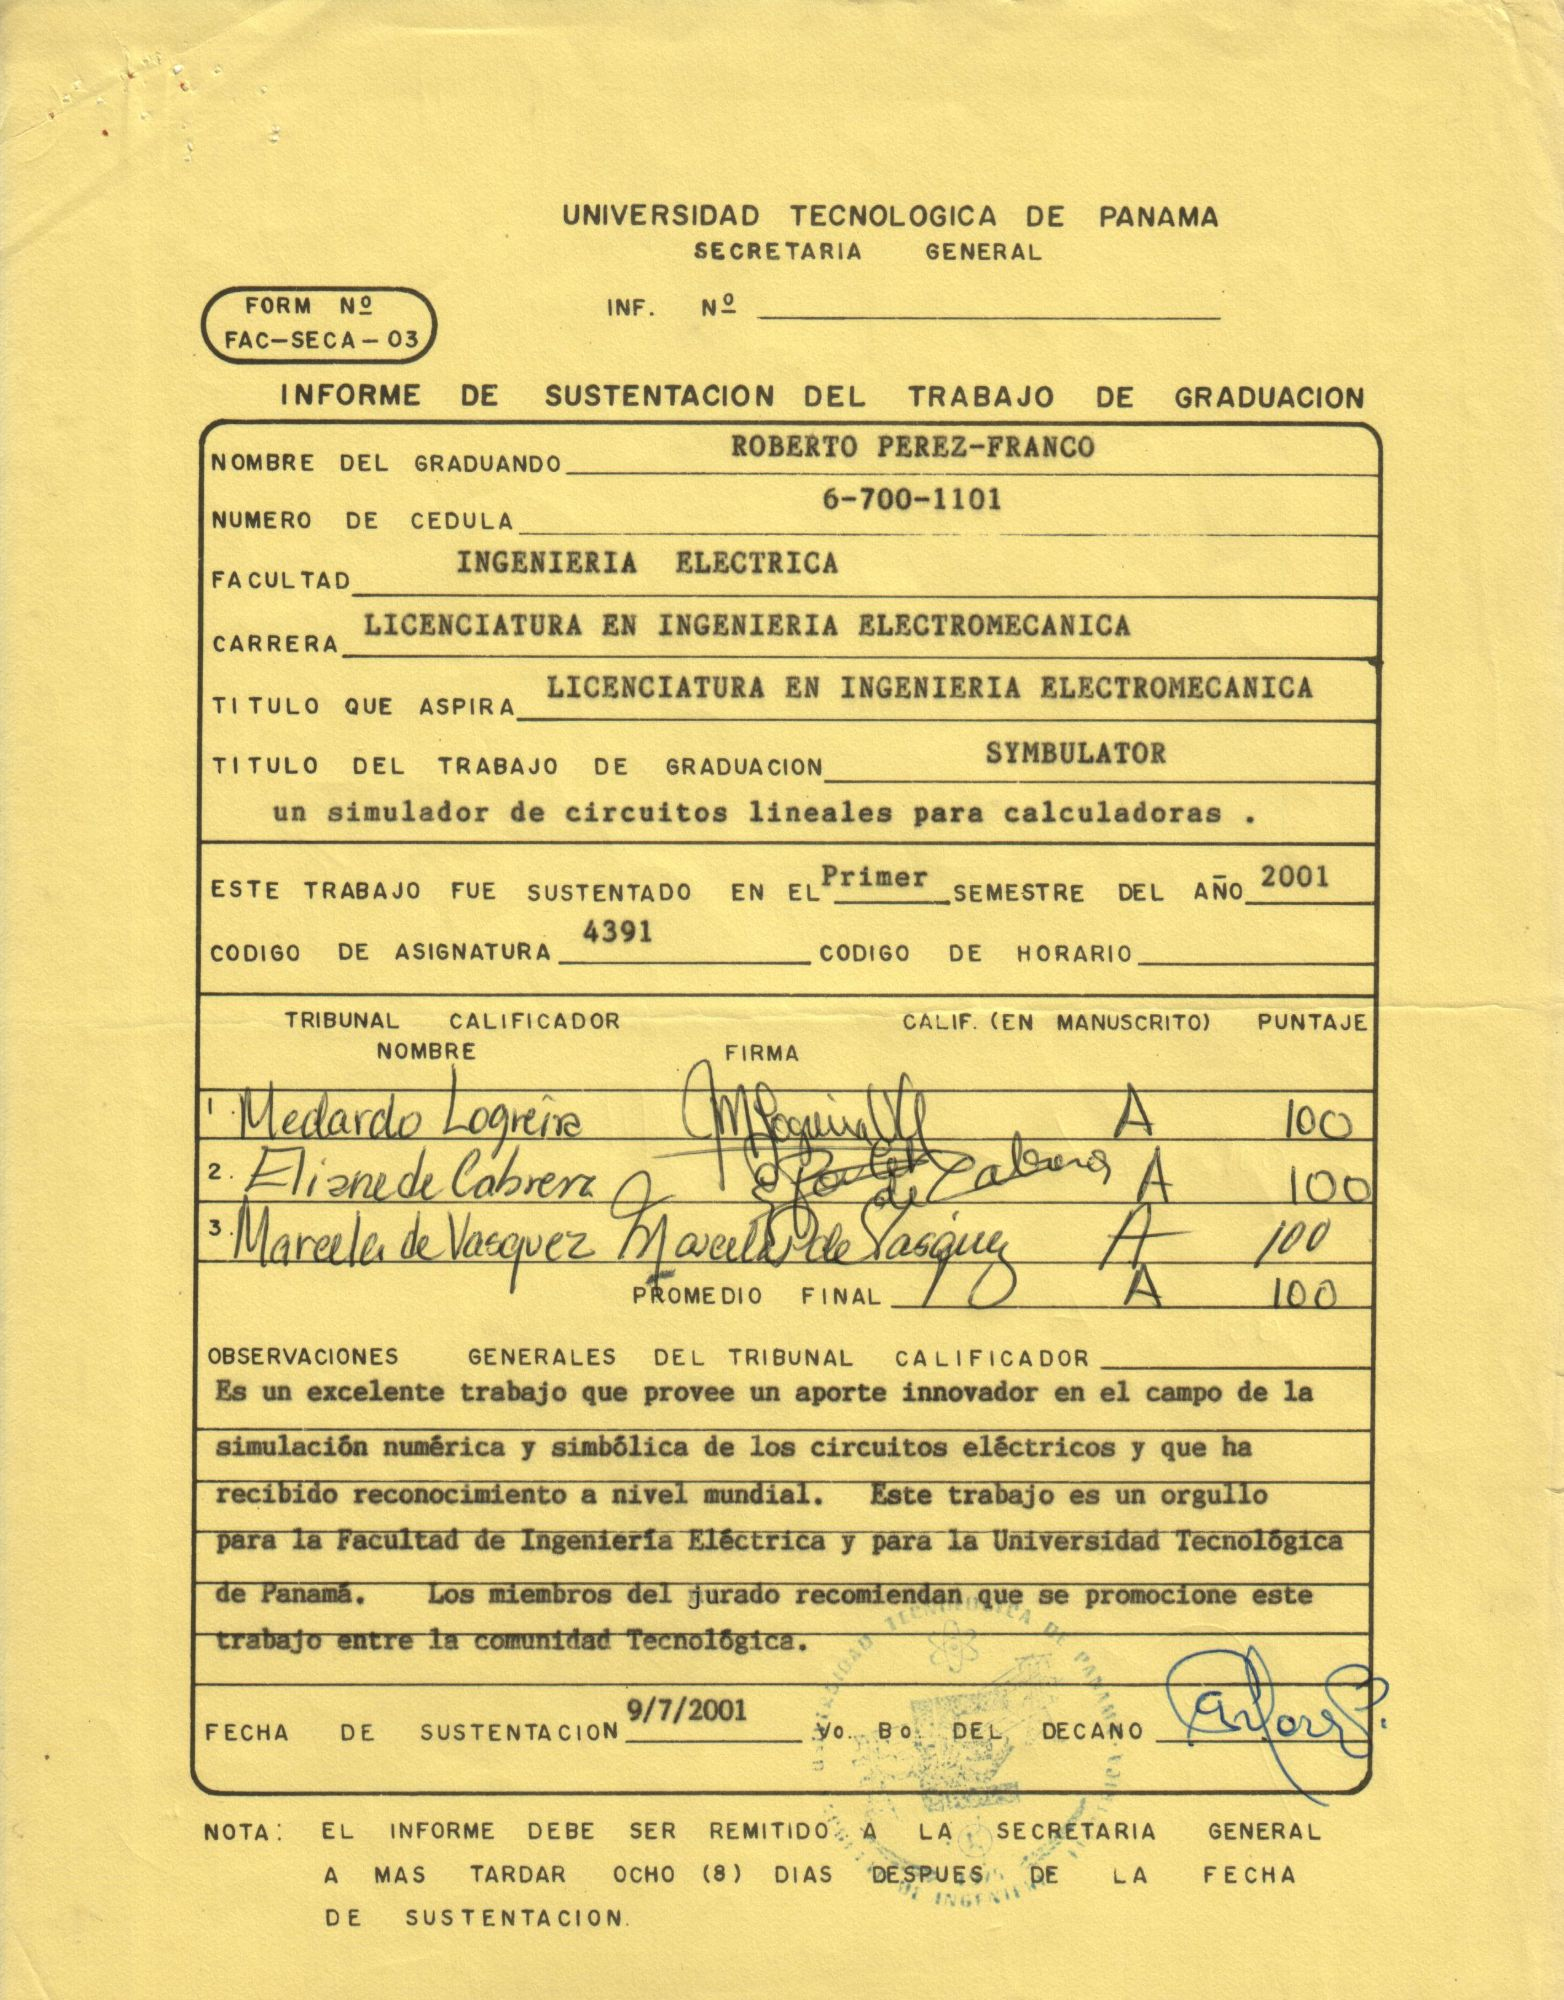
\includegraphics[width=0.88\textwidth]{references/2001_jury_record.jpg}
\caption{The jury record of the thesis defense, 9 July 2001:
three grades of 100/100, and the tribunal's citation.}
\label{fig:jury}
\end{figure}

\begin{figure}[p]
\centering
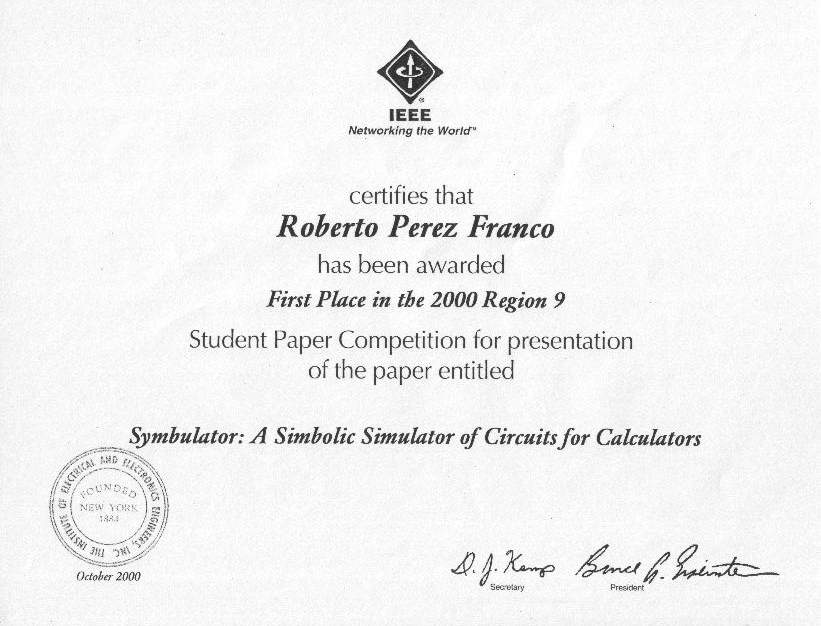
\includegraphics[width=\textwidth]{references/2000_ieee_award.jpg}
\caption{First Place, IEEE Region 9 Student Paper Competition, 2000.}
\label{fig:ieee}
\end{figure}

% ======================================================================
\chapter{The exemplar circuits, drawn}
\label{app:schematics}
% ======================================================================

The schematics below are not illustrations prepared for this
monograph: each one was \emph{drawn by Symbulator~9's schematic
engine} from the same circuit description that
Chapter~\ref{ch:exemplars} solves, exactly as the app draws a
circuit beside its answers. The conventions are the drawer's own:
wires never cross an element body, genuine crossings are drawn as
semicircular hops, junction dots sit on node corners, values read as
the user typed them, and a dependent source carries its controlling
expression as its value.

\begin{figure}[p]
\centering
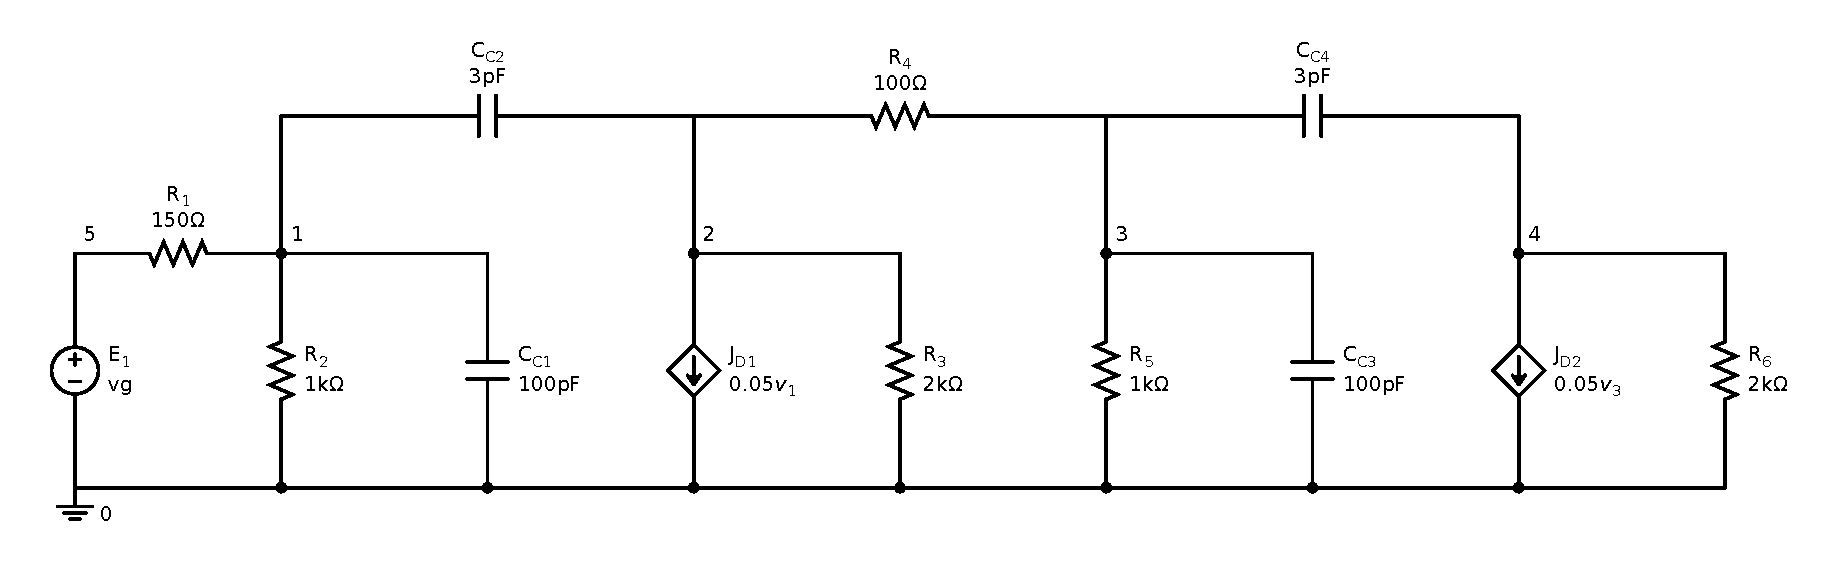
\includegraphics[width=\textwidth]{figures/ex_amplifier.pdf}
\caption{The two-stage amplifier of 1999 (\S\ref{sec:amplifier});
thesis Problem~87.}
\label{fig:ex-amplifier}
\end{figure}

\begin{figure}[p]
\centering
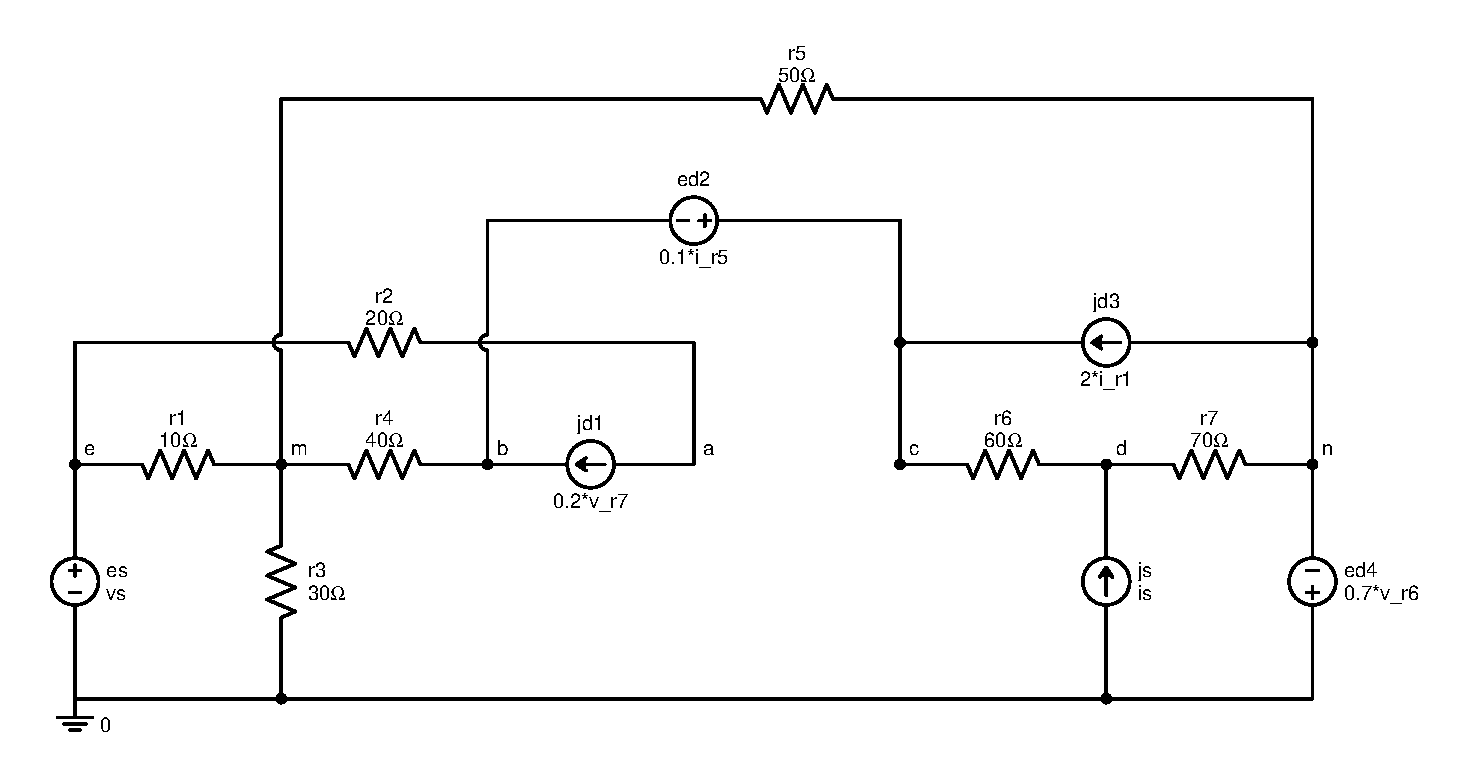
\includegraphics[width=\textwidth]{figures/ex_showcase2013.pdf}
\caption{The 2013 showcase (\S\ref{sec:showcase2013}): one dependent
source of each species, and both independent sources symbolic.}
\label{fig:ex-showcase}
\end{figure}

\begin{figure}[p]
\centering
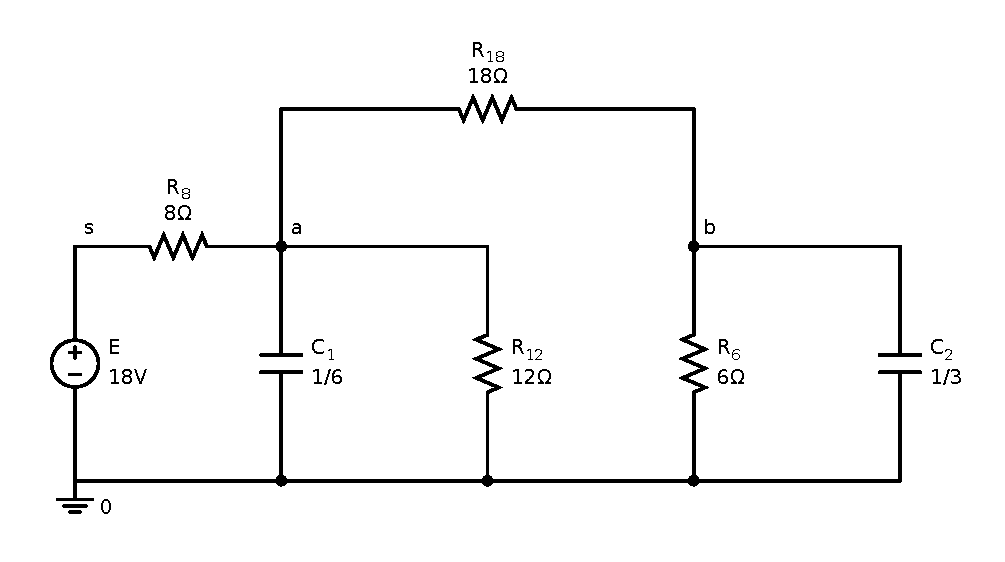
\includegraphics[width=0.62\textwidth]{figures/ex_boulet_before.pdf}\\[2em]
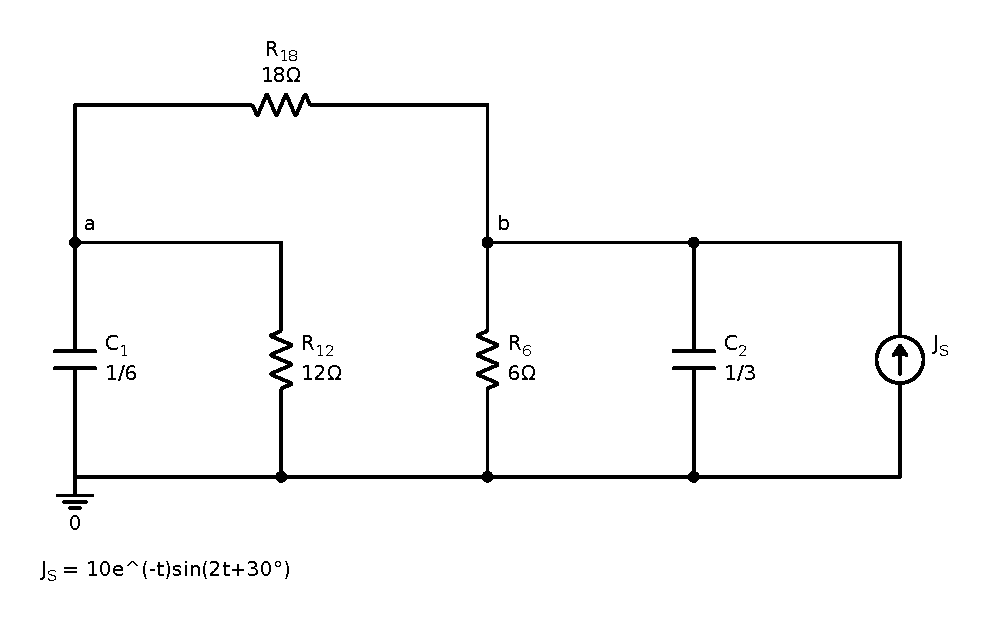
\includegraphics[width=0.62\textwidth]{figures/ex_boulet_after.pdf}
\caption{Prof.\ Boulet's switching transient
(\S\ref{sec:boulet}); thesis Problem~88. Above, the $t<0$ circuit
whose DC solution supplies the initial conditions; below, the $t>0$
circuit carrying them in the capacitors' fifth fields, with the
waveform source connected.}
\label{fig:ex-boulet}
\end{figure}

\begin{figure}[p]
\centering
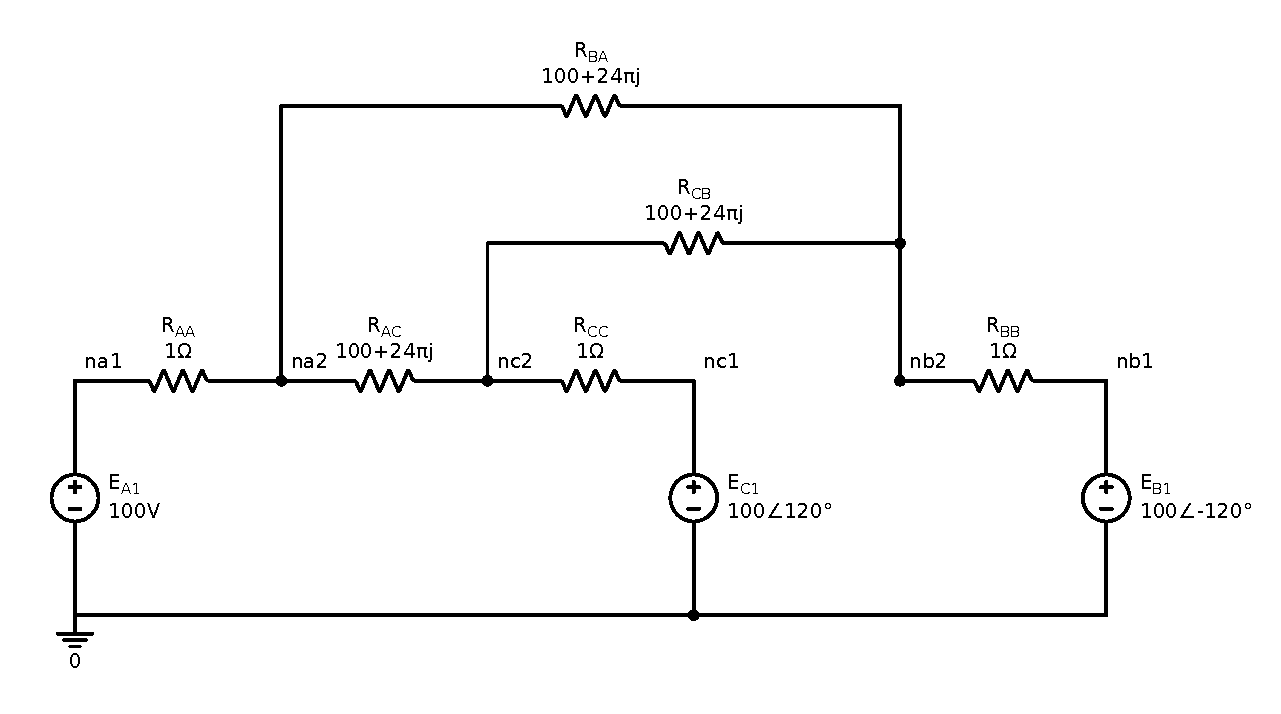
\includegraphics[width=0.9\textwidth]{figures/ex_threephase.pdf}
\caption{The balanced wye--delta system with line impedances
(\S\ref{sec:threephase}), its sources typed in angle notation.}
\label{fig:ex-threephase}
\end{figure}

\begin{figure}[p]
\centering
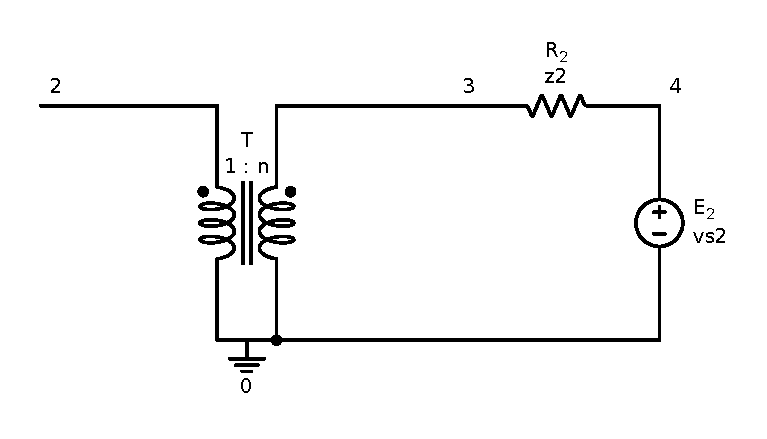
\includegraphics[width=0.55\textwidth]{figures/ex_transformer.pdf}
\caption{The ideal transformer viewed from its primary
(\S\ref{sec:transformer}), every value a symbol.}
\label{fig:ex-transformer}

\vspace{3em}

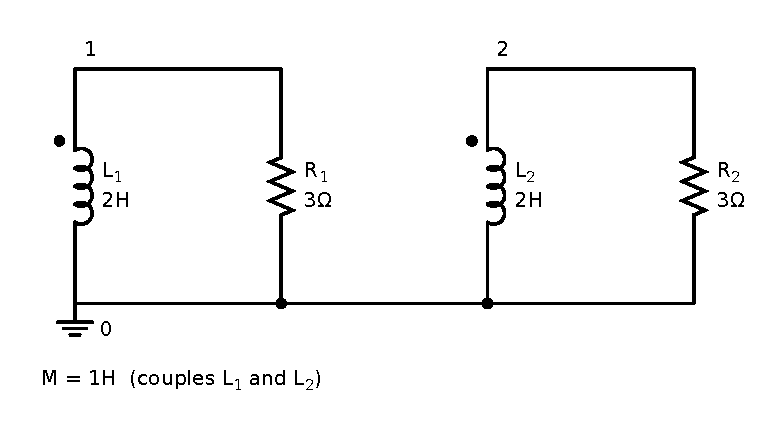
\includegraphics[width=0.5\textwidth]{figures/ex_coupledcoils.pdf}
\caption{The coupled coils with an initial current
(\S\ref{sec:coupledcoils}).}
\label{fig:ex-coupledcoils}
\end{figure}

\begin{figure}[p]
\centering
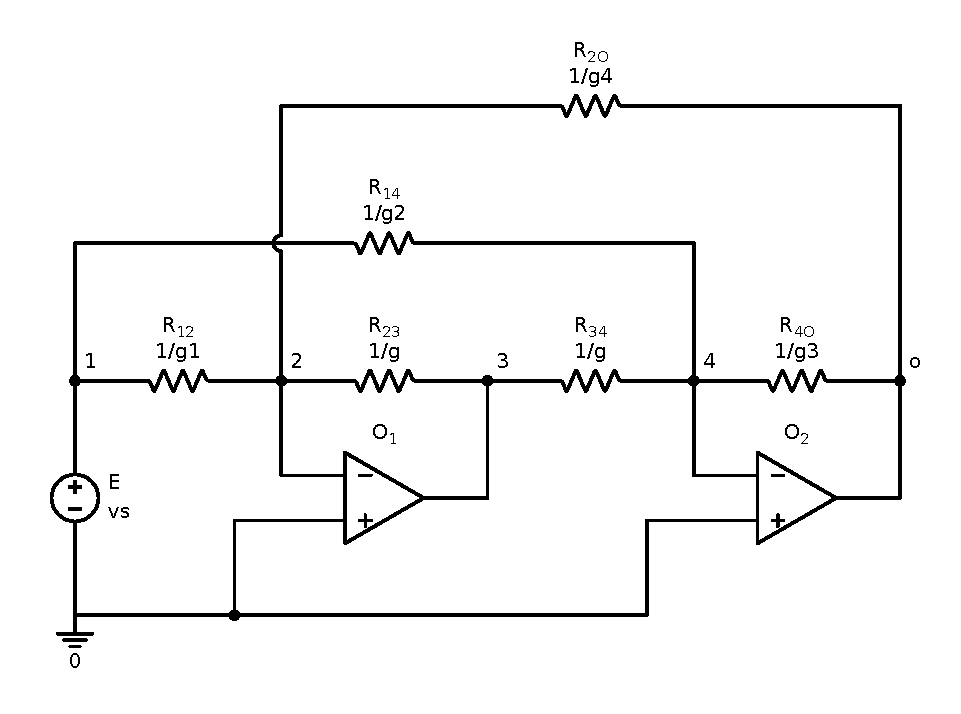
\includegraphics[width=0.85\textwidth]{figures/ex_twoopamps.pdf}
\caption{The all-symbolic two-op-amp cascade
(\S\ref{sec:twoopamps}).}
\label{fig:ex-twoopamps}
\end{figure}

% ======================================================================
% Back matter
% ======================================================================

\section*{Acknowledgments}
\addcontentsline{toc}{chapter}{Acknowledgments}

Symbulator 9 is built on Python and SymPy, and Symbulator's author
thanks their
creators and maintainers. Versions 7 and 8's Laplace transforms are
due to Lars Frederiksen, adapted for the TI-Nspire by Philippe Fortin.
Over the decades, many users improved Symbulator through suggestions
and corrections; they are acknowledged individually in the Symbulator
documentation. The teaching corpus draws its problems from widely used
circuit analysis textbooks, credited in full in the documentation.

\begin{thebibliography}{9}
\addcontentsline{toc}{chapter}{Bibliography}

\bibitem{paper1999}
R.~Perez-Franco (under the pseudonym \emph{Th\'evenin}),
``Symbulator: simulador simb\'olico de circuitos lineales para
calculadoras,'' competition paper, IEEE Student Paper Contest for
Latin America, Nov.\ 1999 (first place, 2000). English translation:
``Symbulator: the calculator-based symbolic circuit simulator.''
Both preserved in this monograph's \code{references/} archive.

\bibitem{thesis2000}
R.~P\'erez-Franco, \emph{Symbulator: un simulador de circuitos
lineales para calculadoras}, Trabajo de Graduaci\'on (Licenciatura en
Ingenier\'ia Electromec\'anica), Universidad Tecnol\'ogica de
Panam\'a, written 2000--2001, defended 9~July 2001 (graded 100/100;
jury record in Appendix~\ref{app:documents}). Twelve chapters and
four appendices; 89 worked problems with provenance. Both the
Spanish original and the surviving 2001 translation fragments are
preserved in this monograph's \code{references/} archive
(\code{2000\_thesis/}, \code{2000\_thesis/english\_translation/});
for the completed English edition, see~\cite{book2026}.

\bibitem{book2026}
R.~P\'erez-Franco, \emph{The Symbulator Book: A Linear Circuit
Simulator for Calculators}, the completed English edition of the
2001 thesis~\cite{thesis2000}. Preface, notice, and chapters~1--4
translated by D.~Burkett and T.~Hutcheson (ca.~2001); chapters
5--12, back matter, and appendices translated by Claude (2026) in
the same voice. Published alongside this monograph. [Online].
Available: \url{https://learn.symbulator.com/book.pdf}

\bibitem{website2001}
R.~Perez-Franco, \emph{Symbulator: Symbolic Circuit Simulator ---
on-line documentation}, 2001 website (introduction, instructions,
expert-mode, Impala-mode, tools, and examples pages), documenting
Symbulator~Q (version~5) and \emph{The Symbulator Book} (12 chapters,
in Spanish; chs.\ 1--4 translated by T.~Hutcheson and D.~Burkett).
Preserved in this monograph's \code{references/} archive.

\bibitem{book2014}
R.~Perez-Franco, \emph{The Symbulator Book}, unfinished English
edition, ca.\ 2014, documenting Symbulator~6. Preserved in this
monograph's \code{references/} archive.

\bibitem{fragment2014}
R.~Perez-Franco, ``Symbolic simulation of linear circuits with
Symbulator,'' unpublished fragment, ca.\ 2014. Preserved in this
monograph's \code{references/} archive.

\bibitem{symbulator-site}
R.~Perez-Franco, \emph{Symbulator: symbolic simulation of linear
circuits}. [Online]. Available: \url{https://symbulator.com}

\bibitem{symbulator-docs}
R.~Perez-Franco, \emph{The Symbulator 9 Documentation}. [Online].
Available: \url{https://learn.symbulator.com}

\bibitem{sympy}
A.~Meurer \emph{et~al.}, ``SymPy: symbolic computing in Python,''
\emph{PeerJ Computer Science}, vol.~3, p.~e103, 2017.

\bibitem{alexander}
C.~K. Alexander and M.~N.~O. Sadiku, \emph{Fundamentals of Electric
Circuits}, 7th~ed. New York: McGraw-Hill, 2020.

\bibitem{bobrow}
L.~S. Bobrow, \emph{Elementary Linear Circuit Analysis}, 2nd~ed.
Oxford: Oxford Univ.\ Press, 1987.

\bibitem{thomas}
R.~E. Thomas, A.~J. Rosa, and G.~J. Toussaint, \emph{The Analysis and
Design of Linear Circuits}, 5th~ed. Hoboken: Wiley, 2006.

\end{thebibliography}

\end{document}
